\documentclass[final,authoryear,5p,times,twocolumn]{elsarticle}
%\documentclass[authoryear,preprint,review,12pt]{elsarticle}

%\usepackage{epstopdf}
\usepackage{graphicx}
\usepackage{amssymb}
\usepackage[pdftex,pdfpagemode={UseOutlines},bookmarks,bookmarksopen,colorlinks,linkcolor={blue},citecolor={green},urlcolor={red}]{hyperref}
\usepackage{hypernat}
%\usepackage{url}
\usepackage{upquote}
\usepackage{upgreek}

\journal{Astronomy \& Computing}

\begin{document}
\begin{frontmatter}

\title{Spectroscopic Analysis in the Virtual Observatory Environment with SPLAT-VO}

\author[OND]{Petr \v{S}koda\corref{cor1}}
\ead{skoda@sunstel.asu.cas.cz}
\author[DUR]{Peter W. Draper}
\author[HDB]{Margarida Castro Neves}
\author[VSB]{David Andre\v{s}i\v{c}}
\author[COR]{Tim Jenness}
\cortext[cor1]{Corresponding author}

\address[OND]{Astronomical Institute of the Academy of Sciences,Fri\v{c}ova~298, 251\,65, Ond\v{r}ejov, Czech Republic}
\address[DUR]{Department of Physics, Institute for Computational
Cosmology, University of Durham, South Road, Durham DH1 3LE, UK}
\address[HDB]{Universit\"a{}t Heidelberg, Astronomisches Rechen-Institut,
M\"o{}nchhofstra\ss{}e 12--14, 69120 Heidelberg, Germany}
\address[VSB]{Department of Computer Science, Faculty of Electrical
Engineering and Computer Science, V\v{S}B --- Technical University of Ostrava\\
 17. listopadu 15, 708 33 Ostrava-Poruba, Czech Republic}
\address[COR]{Department of Astronomy, Cornell University, Ithaca, NY 14853, USA}


\begin{abstract}
  SPLAT-VO is a powerful graphical tool for displaying, comparing, modifying
  and analysing astronomical spectra, as well as searching and retrieving
  spectra from services around the world using Virtual Observatory (VO)
  protocols and services. The development of SPLAT-VO started in 1999, as part
  of the Starlink STARJAVA initiative, sometime before that of the VO, so
  initial support for the VO was necessarily added once VO standards and
  services became available. Further developments were supported by the JAC,
  Hawaii until 2009. Since end of 2011 development of SPLAT-VO has been
  continued by the German Astrophysical Virtual Observatory, and the
  Astronomical Institute of the Academy of Sciences of the Czech Republic.
  From this time several new features have been added, including support for
  the latest VO protocols, along with new visualisation and spectra storing
  capabilities. This paper presents the history of SPLAT-VO, it's
  capabilities, recent additions and future plans, as well as a discussion on
  the motivations and lessons learned up to now.
\end{abstract}
\begin{keyword}
Spectral Analysis \sep Virtual Observatory \sep VO \sep SPLAT-VO \sep STARJAVA
\end{keyword}
\end{frontmatter}

%% Local commands

\newcommand{\qjras}{QJRAS}
\newcommand{\apj}{ApJ}
\newcommand{\aap}{A\&A}
\newcommand{\aspconf}{ASP Conf.\ Ser.}

%% Links
\newcommand{\ascl}[1]{\href{http://www.ascl.net/#1}{ascl:#1}}

%-------------------------------------------------------
\section{Introduction}

There are many tools for the analysis of astronomical spectra.  The most
commonly used of these are the various packages of MIDAS
\citep[][\ascl{1302.017}]{1992ASPC...25..115W}, IRAF
\citep[][\ascl{9911.002}]{2012ASPC..461..595F}, Starlink
\citep[][\ascl{1110.012}]{1982QJRAS..23..485D}, together with many IDL
extensions and scripts. Very advanced processing is still often done in custom
(especially FORTRAN) programs used by small communities.  These tools tend to
work with specially formatted files (quite often ASCII tables) stored on local
disks.

The common tasks of an astronomer during spectral analysis consists of finding
the required spectra in various archives, downloading them, understanding and
extracting the metadata (e.g.\ date of exposure, spectral range, flux units),
converting to the custom format used by the particular tool, visualizing
selected spectra and  removing the bad ones (e.g.\ noisy). Then he can finally
run some massive processing (and measurement of various parameters) on an
improved list.  Very often is the measurement of some variables (e.g. radial
velocity or equivalent widths of selected lines) accomplished interactively
and the spectra must be zoomed and unzoomed, panned, rescaled etc.

It is seen that a real scientific analysis of thousands of spectra is a very
tedious task even on the same instrument. But the real modern challenge is an
analysis of multi-wavelength spectra from different instruments, where all the
metadata are different, there are various flux and wavelength, frequency or
energy units  and where the formats of storage also vary (simple FITS, binary
tables, ASCII lists etc.).

To make the handling of spectra obtained from world-wide distributed
heterogeneous archives simple and efficient was the main motivation for
developing the International Virtual Observatory Alliance Simple Spectra
Access Protocol \citep[IVOA SSAP;][]{ssap}. The key elements of this
http-based protocol is the the standard spectra discovery mechanism (like a
Google for astronomical data) called IVOA Registry \citep{registry} and  the
standard data format called VOTable \citep{2004tivo.conf..118O},
describing the metadata of retrieved spectra in a limited vocabulary of
obligatory parameters.

  \subsection{The SSA Protocol}
%
SSAP allows the astronomer to find all the world-wide VO-compatible archival
spectra of his favourite object, it can also be used to get spectra for all
the objects in a `circular' region of interest on the sky. These simple
queries can be refined using spectral ranges, dates of observation as well as
subject to more subtle criteria like spectral resolution or target class (even
spectral type) if the server supports such refinement. More capable servers
provide extended facilities for converting spectra on-the-fly to the required
format (and in principle can create e.g. previews of spectra in PNG or deliver
the fluxes and wavelengths in ASCII or CSV tables).

\subsection{SSAP-compatible  Visualization Clients}
%
Although a regular work with large amounts of data is more convenient by
calling the SSAP protocol from some scripting language in a batch like or
workflow-based environment, the crucial feature for understanding data is the
advanced visualization and comfortable user interaction.  Therefore the very
important part of the VO infrastructure represent the VO-compatible spectra
visualization clients.  So far there are there three of them.

VOSpec \citep[][\ascl{1205.011}]{2005ASPC..347..198O}, developed by ESA, is
designed strictly on principles of IVOA standards and was rather focused on
analysis of high energy and space-based spectra with absolute flux
calibration, lacking support for some common functions and custom data formats
used in ground-based stellar spectroscopy. The most critical 1D FITS image
format was added just recently. VOSpec contains quite complex non-linear
model-fitting package and can handle the photometric points as well as Spectra
Energy Distributions (SEDs).

The two other clients are in fact the former general spectra analysis tools
with built-in separate plugin for querying and downloading spectra using SSAP.
The advantage of this approach is the support for many legacy data formats and
various domain-specific functionality, better tuned to requirements of
scientists not familiar with VO technology.

Specview \citep[][\ascl{1210.016}]{2002SPIE.4847..410B}, developed at STScI,
was intended mainly for handling spectra from Hubble Space Telescope
instrumentation and some other NASA missions, but gradually transformed into
VO-compatible general client supplemented with a library of theoretical
spectra and various models for SED generation.  While the Specview is very
powerful tool  compatible with a lot of very special formats from HST, IUE,
FUSE, ISO and GALEX  satellites, allowing the advanced comparison of
observations with a wide range of theoretical spectra models (e.g.\ power
laws, Bremstrahlung,  emission line profiles,  interstellar extinction, dusty
rings or  whole Kurucz library of spectral types), it is less flexible in
support of various SSAP features and lacking behind the rapid IVOA standards
evolution.

In contrast with it, the last VO-compatible client for spectra analysis,
SPLAT-VO \citep[][\ascl{1402.008}]{sun243} was revived recently and currently
is under intensive development serving as a test-bed for newly proposed VO
standards and special features.


%\subsection{VO access in practical examples}

%-------------------------------------------------------

\section{History of SPLAT-VO}
\subsection{Genesis}

The SPLAT-VO project is an extension to an older one simply called
SPLAT \citep[][\ascl{1402.007}]{2002ASPC..281..513B}.  The name SPLAT
is based on the words SPectraL Analysis Tool, an application for the
display and analysis of spectral data. The development of SPLAT itself
was started by the Starlink Project \citep{1982QJRAS..23..485D} in
1999 in response to a perceived need within the UK astronomy community
for a spectral domain tool with capabilities similar to those of the
successful GAIA tool \citep[][\ascl{1403.024}]{2000ASPC..216..615D}
that supported imaging data. SPLAT was also a leader project for
moving future developments into the Java language, with the obvious
benefits of improved portability, modern language capabilities (OOD,
OOP) and core-level support for features like UIs and internet
protocols and services. This work eventually led to the formation of
what became the STARJAVA project, now hosted at
\url{https:://github/Starlink/starjava}, where the source code for
SPLAT-VO and other STARJAVA projects, like TOPCAT
\citep[][\ascl{1101.010}]{2005ASPC..347...29T}, can be freely
downloaded.

\subsection{SPLAT-VO}

The first VO capabilities added to SPLAT where released in 2005
\citep{2005ASPC..347...22D}, as support for querying VO registries for
Simple Spectral Access Protocol servers was added. A selection of
these servers could then be queried for any spectra they contained
within a region on the sky and these could then be selected and
displayed. SPLAT already had the ability to match a wide range of
spectral coordinate systems and flux units, so the spectra could be
displayed within the same plots for direct comparison. Since then SSAP
support has been developed further with version 1 of the standard and
various enhancements like being able to query for an object, not just
a region.

The second phase of VO developments in SPLAT-VO were the incorporation
into the VO-desktop, so that spectra and tables could be shared
between applications.  Initially, in 2006, this used the PLASTIC
\citep{2007ASPC..376..511T} protocol and more latterly SAMP
\citep{2012ASPC..461..279T}.

More recently, in 2011, the VO aspects of SPLAT-VO have been taken over by Margarida
Castro Neves, from the German Astrophysical Virtual Observatory (GAVO) in
Heidelberg, Germany.  Due to the need for a spectral domain application with
VO capabilities and good scientific analysis functions, GAVO  decided to resume
its development once the original funding had stopped. In this way SPLAT-VO can
continue to be improved, and kept up-to-date with the changing requirements of
both end users and data providers.  This development  is done in cooperation
with Petr \v{S}koda (Astronomical Institute of the Academy of Sciences of the
Czech Republic), who contributes in defining the user requirements and
suggesting modifications of scientific functions (with emphasis put on optical
stellar spectroscopy of  emission line stars).  His Master and former
Bachelor student David Andre\v{s}i\v{c} from Technical University, Ostrava has been
implementing new analytic functionality (see section.~\ref{davids_functions}) since 2012.

\section{SPLAT-VO Internals}

\subsection{Data Formats}

The SPLAT-VO spectral data model is specified by a single internal interface
that is concretely implemented for the various data formats that are
supported. Having a single interface decouples the data model and makes it
practical to support a wide range of formats, but necessarily means that some
format specific features will not be supported and can be lost when making
transformative changes like saving back to file.

The SPLAT-VO data model is simple only requiring that spectra have a name,
coordinate system and some data values. Other supported items are data errors,
fuller descriptions, keyed properties (key, value, description), data units
and labels, and the underlying dimensionality (if the spectrum is being
extracted from a 2D or 3D array). Spectra can also have mutable properties,
like the names of the table columns that contain the various data values.

Current implementations give SPLAT-VO access to spectra in simple text
files, FITS \citep{2010A&A...524A..42P}, NDF \citep{ndfjenness}, NDX
\citep{2003ASPC..295..221G}, as well as FITS and VO tables. Tables are
supported using the STILTS
\citep[][\ascl{1105.001}]{2006ASPC..351..666T} library. In addition to
these spectra can also be memory based so that they can become
modifiable and be derived from data with higher dimensionalities.

\subsection{Internal spectral handling}

The presentation of all data types through a single interface works especially
well when coupled with a further, higher-level, abstraction class. This
abstraction is in effect how all the analysis and visualisation code
throughout SPLAT-VO see a `spectrum' (these two elements that decouple an
abstraction from the underlying implementations are in fact the well
established `Bridge Pattern').

This use of a single abstraction to all data formats makes it easier to write
consistent code and extend the basic internal spectrum with new facilities
(methods that do things like extraction sections, replace BAD values etc.) as
well as associate useful properties like graphics and formatting rendering
hints, data and coordinate range limits. Extending the underlying model is
also easy as new features strictly need only be handled in the abstraction
(although clearly that would not be interesting) and new spectral types can
extend the base abstraction (the basic spectral type is extended to also offer
spectra that render as line identifiers and cached copies of remote spectra).


\subsection{Presentation}

The presentation of spectra is based on the model-view-controller pattern that
pervades Java UIs and the same spectral data can be seen and operated on in
many different guises, that is as a number of line plots, tables, property
lists etc. Memory based spectra are also directly modifiable (as simple edits
to table cells or generally using expressions). Through the
model-view-controller infrastructure all changes are propagated to all views.


\subsection{Coordinate systems and units}

Early in the design of SPLAT it was decided that it would not be possible to
replicate the considerable effort that had already been put into a
comprehensive system for handling coordinate systems and units, including full
support for reading and writing FITS WCS \citep{2006A&A...446..747G}. This led to the development of a JNI
library for the Starlink AST library \citep{1998ASPC..145...41W,2012ASPC..461..825B}, JNIAST. AST
itself is written in standard C so compiling it on many platforms is
relatively easy, but, as discussed in Sec.\ \ref{sec:jniast-lesson}, this remains a portability issue at the heart of SPLAT
limiting one of the initial aims.

Some of the advanced features that SPLAT-VO offers based on AST are support
for spectral coordinates in wavelength, velocity, frequency and energy. These
can have standards of rest, so transformations of rest frame are also
supported (important for velocity and laboratory data). SPLAT-VO also supports
double side-band spectra for sub-millimeter spectra and flux unit matching. Many of these features
have been improved in AST over time and SPLAT-VO gains from this.

AST supports all the units specified in the FITS standard
\citep{2010A&A...524A..42P} and can calculate scaling factors to allow
matching of spectra with different flux units. Adding full VOUnits
support \citep{vounits} to SPLAT-VO would currently require that AST
is updated to match the standard. This would have the added benefit of
expanding support for VOUnits to the entire Starlink software
collection and in particular enhance the unit support of the VO
aspects of GAIA \citep{2009ASPC..411..575D}.


\subsection{Scripting of SPLAT-VO}

The various classes of SPLAT-VO may be called directly from the BeanShell
scripting language \citep{niemeyer2013learning}, in principle this allows
complex workflows to be created, and is used to create example scripts that
are part of the standard distribution. These support the batch fitting of
single Gaussian line profiles, as well as composite models consisting of any
number of Gaussian, Lorentzian and Voigt profiles for deblending complex lines
(a feature that has never made it into the full UI). BeanShell scripts are
also used for controlling SPLAT-VO from command line.

%-------------------------------------------------------

\subsection{The Power of SAMP in SPLAT-VO}

Although all SSAP clients have powerful capabilities, they are naturally
limited to their built-in features, which will not suit all the requirements
of a wide spectroscopic community. However, almost all VO-compatible tools,
including important table processor TOPCAT and stellar atlas Aladin
(\ascl{1112.019}), have built-in support for the Simple Application Message
Protocol (SAMP), successor of PLASTIC. This supports the bringing together of
basic VO applications, like bricks, to build complex visualization and
processing pipelines allowing very complicated analyses of truly Big Data.
The astronomer may, for example, visualize the spectra of objects they click
on in some imaging survey frame displayed in Aladin, or identify the visual
appearance of galaxies from the spectra which have been visually selected in
SPLAT-VO.  SAMP was also successfuly used  to send for detailed analysis in
SPLAT-VO  the spectra stored on web server and selected in browser using
their static previews.

\section{SPLAT-VO Capabilities  for Spectra Analysis}

SPLAT-VO as a general purpose spectral analysis tool supports a very wide
range of capabilities required by astronomers for every-day work outside of
the VO. Input spectra may be loaded directly from local disk files in a number
of formats, including several types of multicolumn ASCII tables,
multi-extension FITS with binary tables or 1D spectrum FITS image, as well as
Starlink NDF.

The list of capabilites of SPLAT-VO is enormous and are fully described in
the associated documentation \citep[SUN/243;][]{sun243} which is also
available as online help and includes example data from
multi-wavelength observations.

Here we give a short overview of features not relevant to VO protocols.
Several features are very specific to the analysis of hot emission
line stars.

\begin{itemize}

\item Visual stacking of spectra introducing either constant vertical offset
  or offset based on functions of values of certain FITS keywords. For example
  the line profiles may be ordered by the circular phase computed for a
  certain period. Stacking is also useful for visualization of evolution of
  stellar line profiles in variable stars.  The
  Fig.~\ref{fig:phiper-heros-stack} shows the evolution of an emission line
  profile for the star $\Phi$~Persei observed with HEROS spectrograph at
  Ond\v{r}ejov 2m telescope in years 2001--2003.

\begin{figure*}[t]
\begin{center}
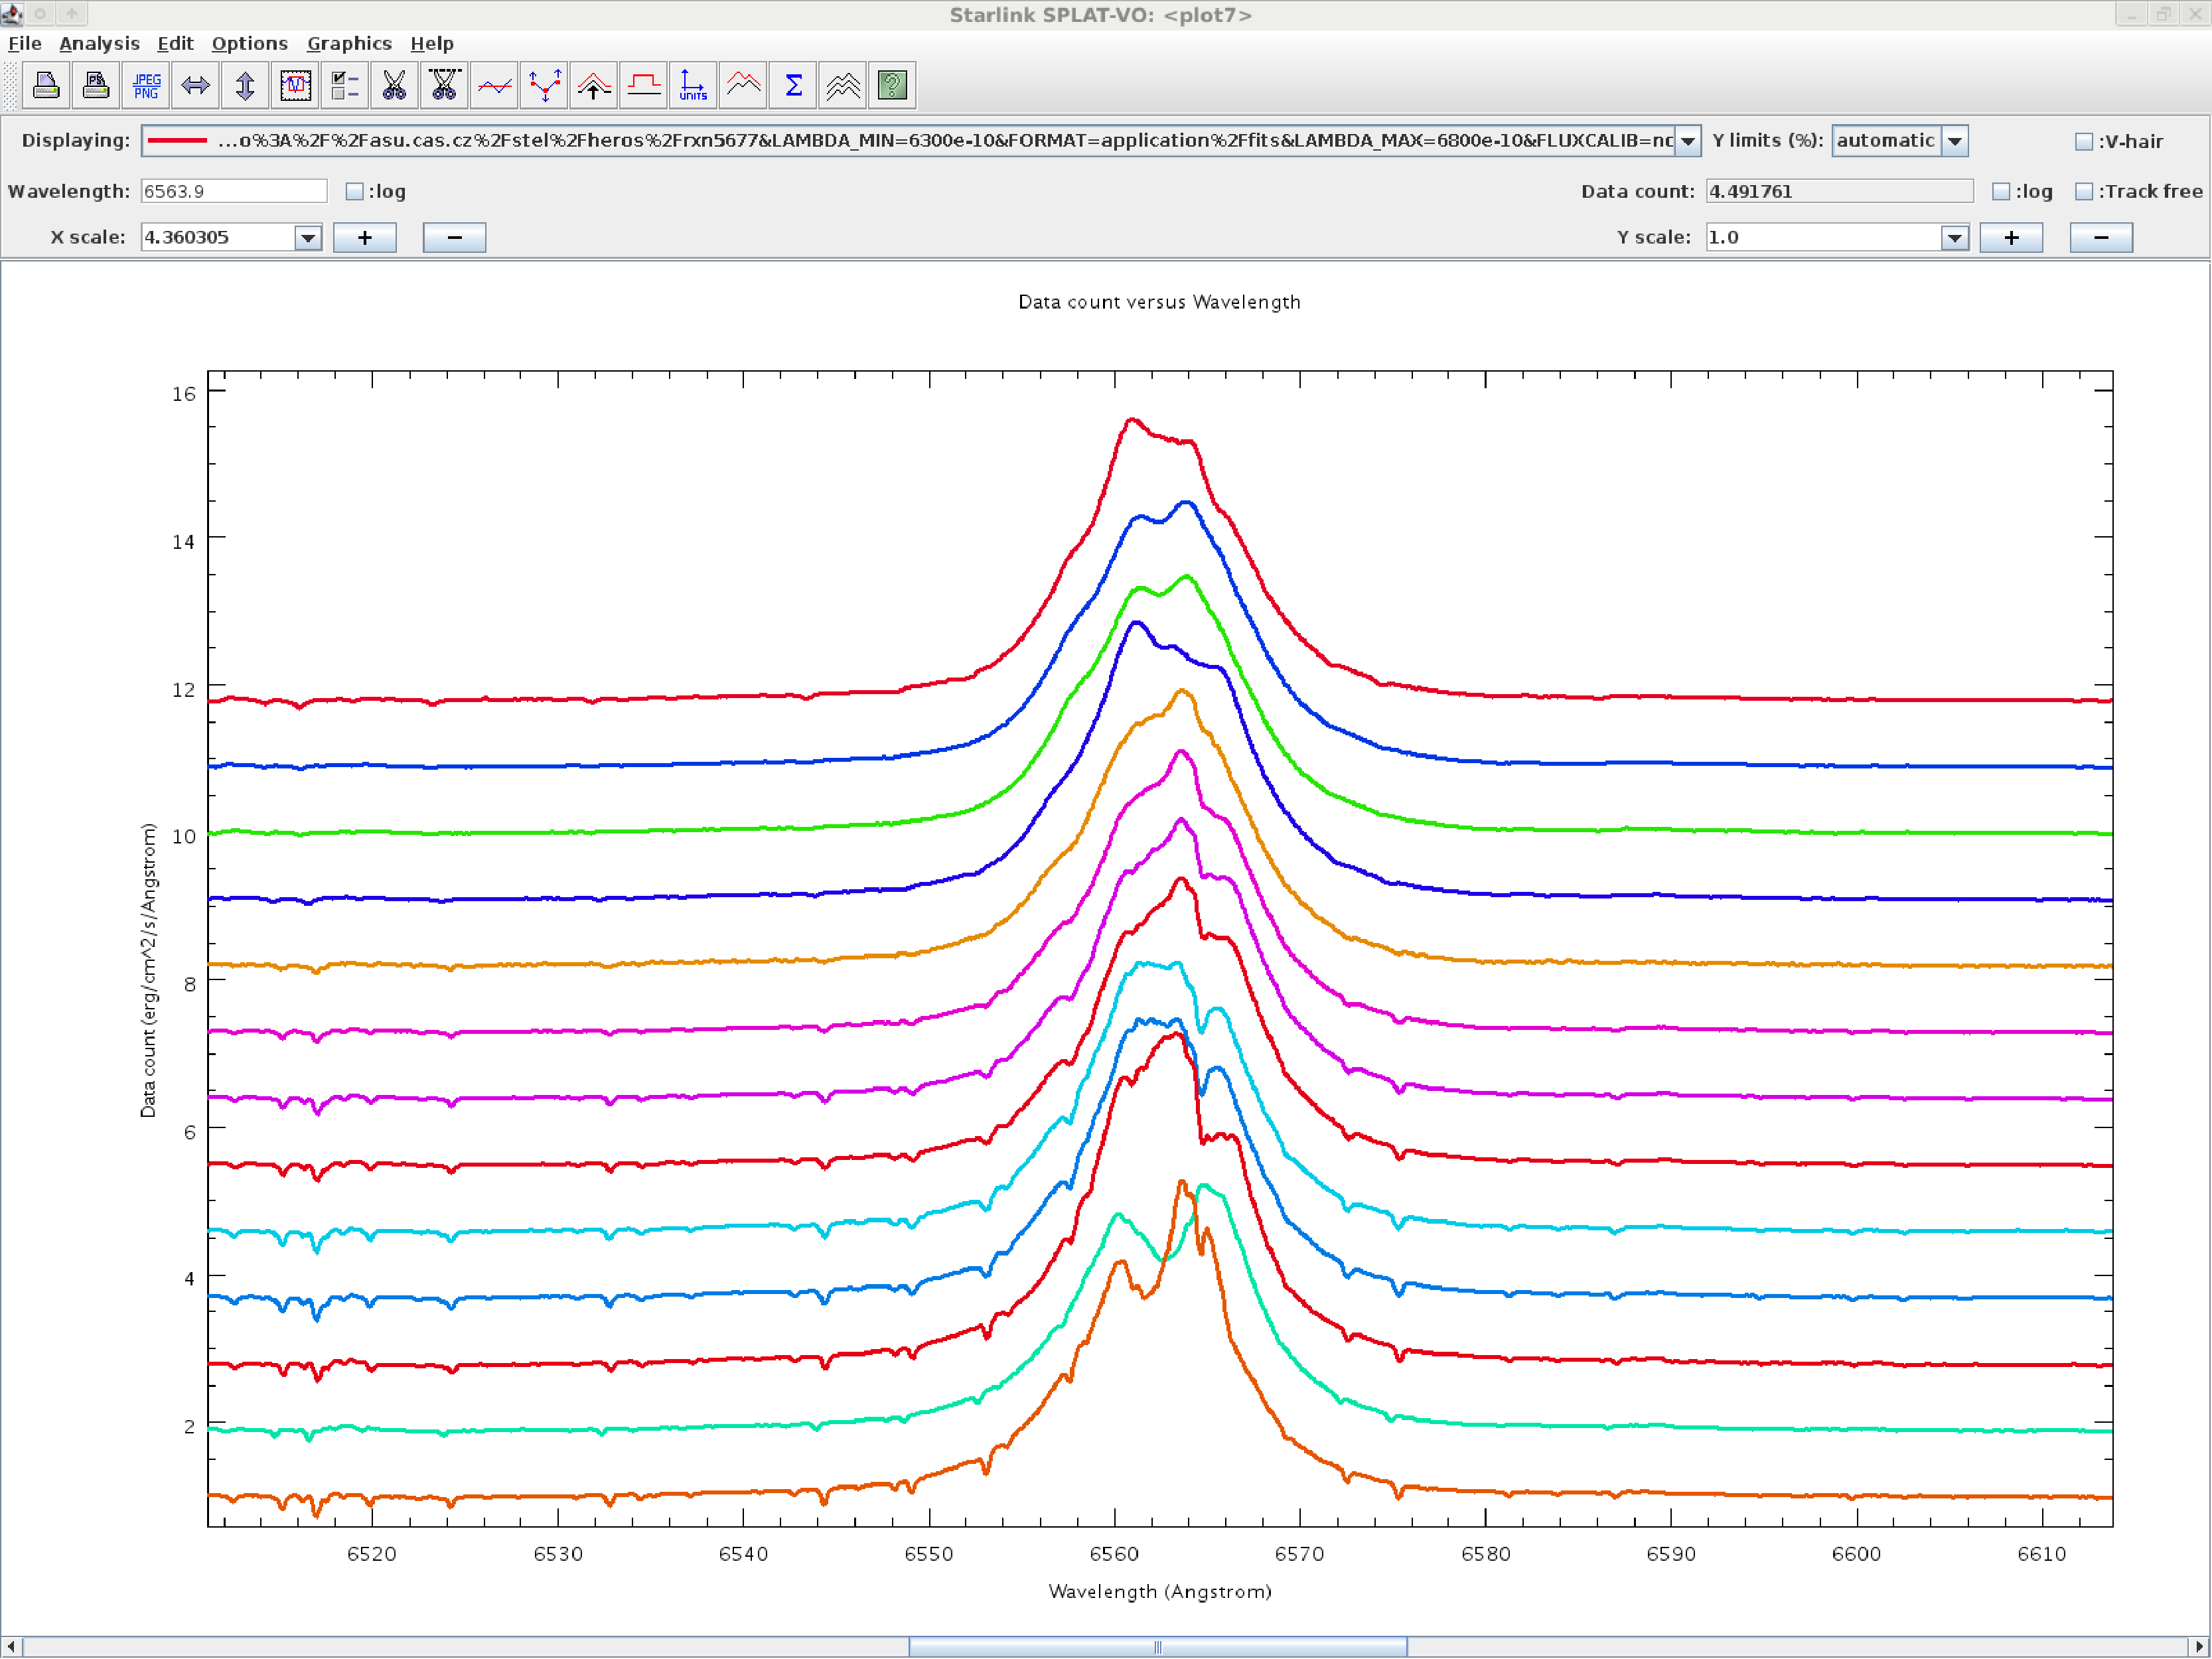
\includegraphics[width=0.8\textwidth]{phiper-heros-stack.pdf}
\caption{The time evolution of the H$_\alpha$ line emission profile in
$\Phi$~Per observations taken using the HEROS spectrograph at Ond\v{r}ejov 2m
telescope. The stacking offset of 0.6  makes sure that the changes can be seen easily}

\label{fig:phiper-heros-stack}
\end{center}
\end{figure*}


\item Measurement of radial velocities by the visual matching of a line
  profile with its mirrored image based on idea of oscilloscopic comparators.
  It is important for measuring the asymmetric and distorted line profiles
  typical for hot emission stars. For detailed explanation see
  \citet{2007IAUS..240..486P}. This feature can be operated with a batch-like
  mode to quick assess a number of lines and or spectra using a `visitor list'.

\item Continuum estimation using flexible curves similar to those expected to
  be drawn by a human. The INTEP procedure based on Hermitean polynomials
  \citep{1982PDAO...16...67H} has been successfully used for decades in
  fitting stellar continua (typically of emission-line stars like Be stars and
  symbiotic ones) in the program SPEFO \citep{1996ASPC..101..187S}. The
  overview of advantages of this procedure is given in
  \citet{2008asvo.proc...97S}. Other curves types are also available such as
  \citet{Akima:1970:NMI:321607.321609}.

\item Powerful transformation of the spectral axis with respect to various
  coordinate systems; air and vacuum wavelength, optical and radio velocities,
  frequency, redshift, energy. The transformations can also include various
  standards of rest; topocentric, heliocentric, dynamic and kinematic local.

\item Built-in spreadsheet processor supported by special astronomical
  functions. Allows the modification/transformation of coordinates and data
  values. Astronomical functions include the spectral profile models.

\item Filtering with smoothing (mean, median, rebin) and denoising with wavelets.

\item Line fitting using Gaussian, Voigt or Lorentz profiles.

\item Statistics of selected regions, mean, median, sum, mode, variance, skew,
      kurtosis, rms, quantiles.

\item Region removal, replacement and extraction. Also replacement part of
spectra  with interpolated curve.

\item Complete graphics toolkit with many configurable options for
  presentation of data. Export of publication quality output in PNG, GIF, EPS.

\item Animation of spectra - creation of slide JPEG/PNG files. Convenient
  for showing the line evolution or non-radial pulsations.

\item Identification of spectral lines using simple supplied ASCII line lists and
 built-in set of common  atomic and molecular lines (includes molecules in sub-millimeter
 region). The Fig.~\ref{fig:zetoph2sp-id} shows the identification of telluric lines on a
 combination of spectra from two different spectrographs of Ond\v{r}ejov 2m
telescope.

\begin{figure*}[t]
\begin{center}
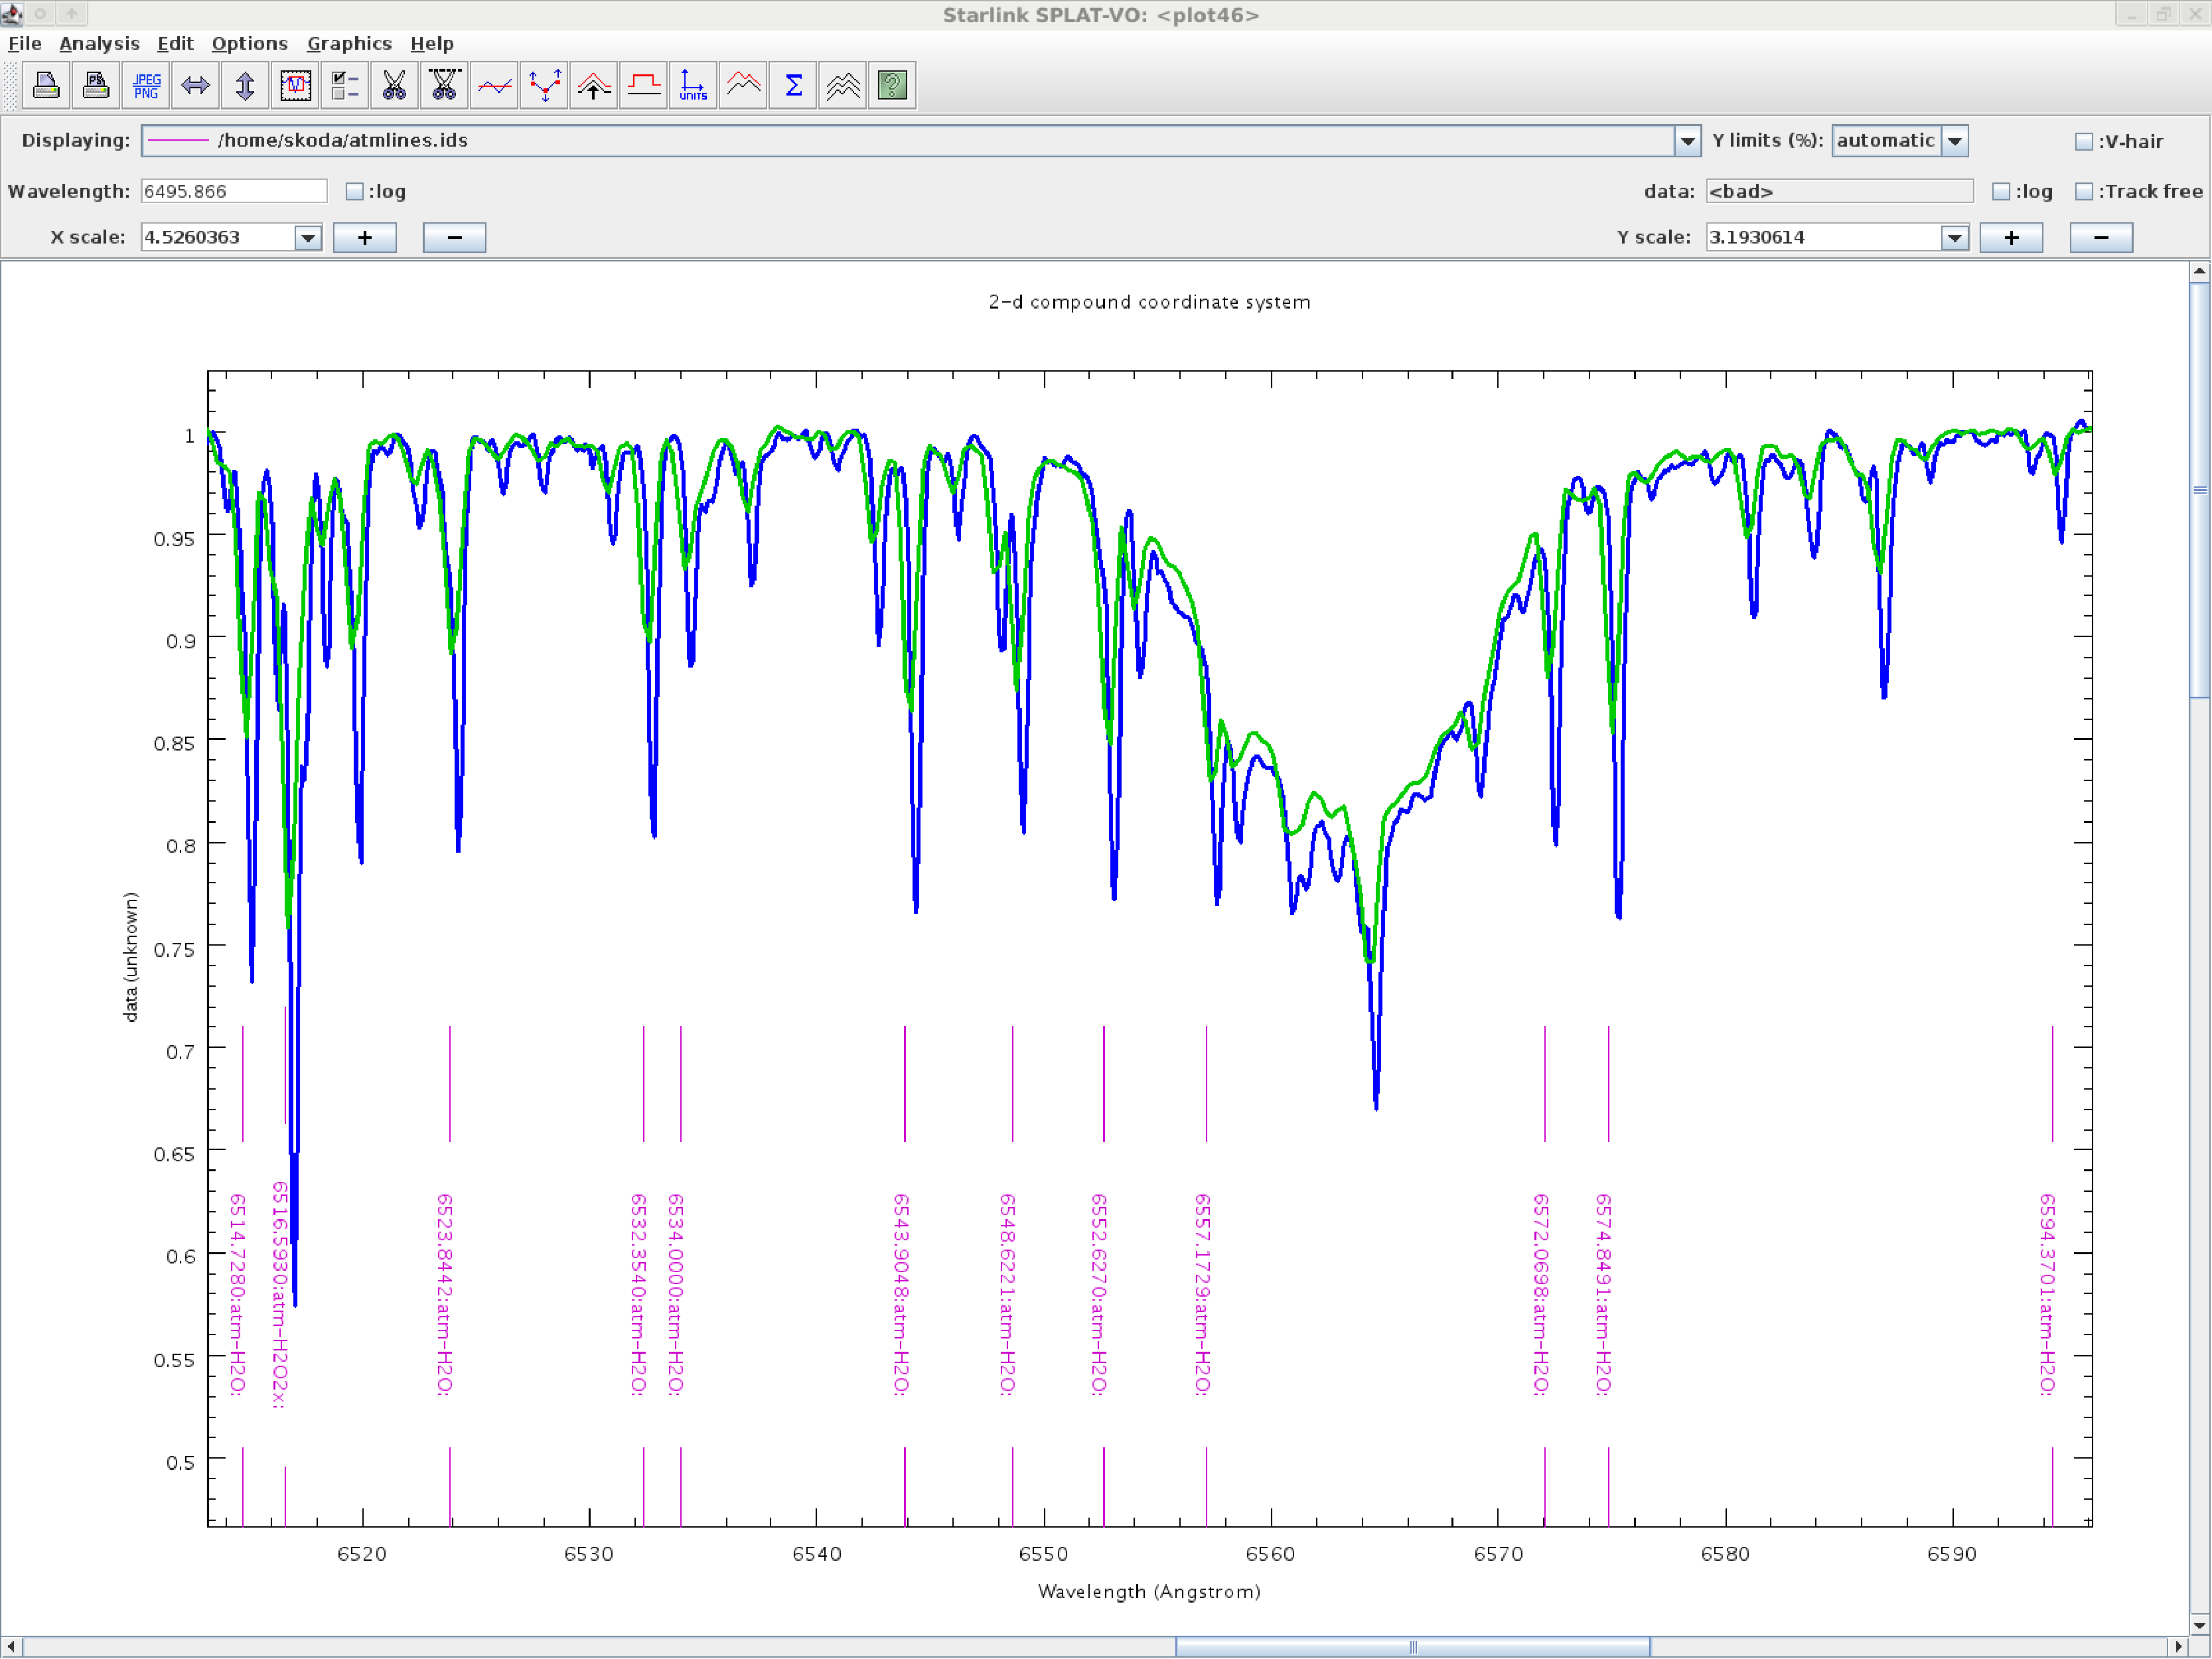
\includegraphics[width=0.8\textwidth]{zetoph2sp-id.pdf}
\caption{Zeta Ophiuchi in H$_\alpha$ region, data obtained with Ond\v{r}ejov Coud\`e
  spectrograph 700mm camera (green) and HEROS spectrograph (blue) with overplotted line
  identification from custom line list of telluric lines. Note the deeper
  telluric lines on HEROS due to its almost double spectral resolving power.}
\label{fig:zetoph2sp-id}
\end{center}
\end{figure*}

\item Simple operations on spectra such as adding, subtracting,
  dividing, and continuum fitting.

\end{itemize}


\section{SPLAT-VO SSAP interface}

The most important for VO funcionality is the SSAP interface, which
has been still in active developing state.  The task of the interface
is to help the user build a correct SSAP query (which is seen
immediately) by filling simple form for parameters like coordinates
({\tt POS}) and size ({\tt SIZE}) of the searching cone of the object
(or name which is translated by CDS names resolver Sesame on request),
spectral ranges ({\tt BAND}), date/time of observation ({\tt TIME}),
status of calibration of wavelength ({\tt WAVECALIB}) and flux ({\tt
  FLUXCALIB}) axis and format ({\tt FORMAT}) of available data.  The
recent addition allows to refine the query using all optional
parameters supported by selected SSAP servers.

The data returned by SSAP server (pointed by {\tt accref} link in
metadata) are loaded onto local computer, stored in a local user's
directory and kept in memory.  Lot of operation can be done afterwards
without SSAP calls on already loaded memory spectra including the
individual tuning of presentation of each spectrum (e.g., line types,
graphics attributes).

The list of SSAP server may be updated using one of selected VO
registries and even the local services not yet registered may be added
manually. The server list may be edited to query only collections with
similar data or even only one service may be queried for detailed
specific operations.

As an example, the Fig.~\ref{fig:hst_query} shows the search of
absolutely calibrated spectra of emission star $\Phi$~Per. We have
selected Hubble Space Telescope with Goddard High Resolution
Spectrograph (at the opened tab, note also the unfolded service
description on the left side) and the IUE low resolution spectra
(selected in other tab).  The composite plot of UV spectra from HST
GHRS (thick blue short pieces) and IUE low resolution spectra (thin
lines - green SWP, pink LWR camera) is on Fig.~\ref{fig:iuehst2}.

\begin{figure*}[Ht]
\begin{center}
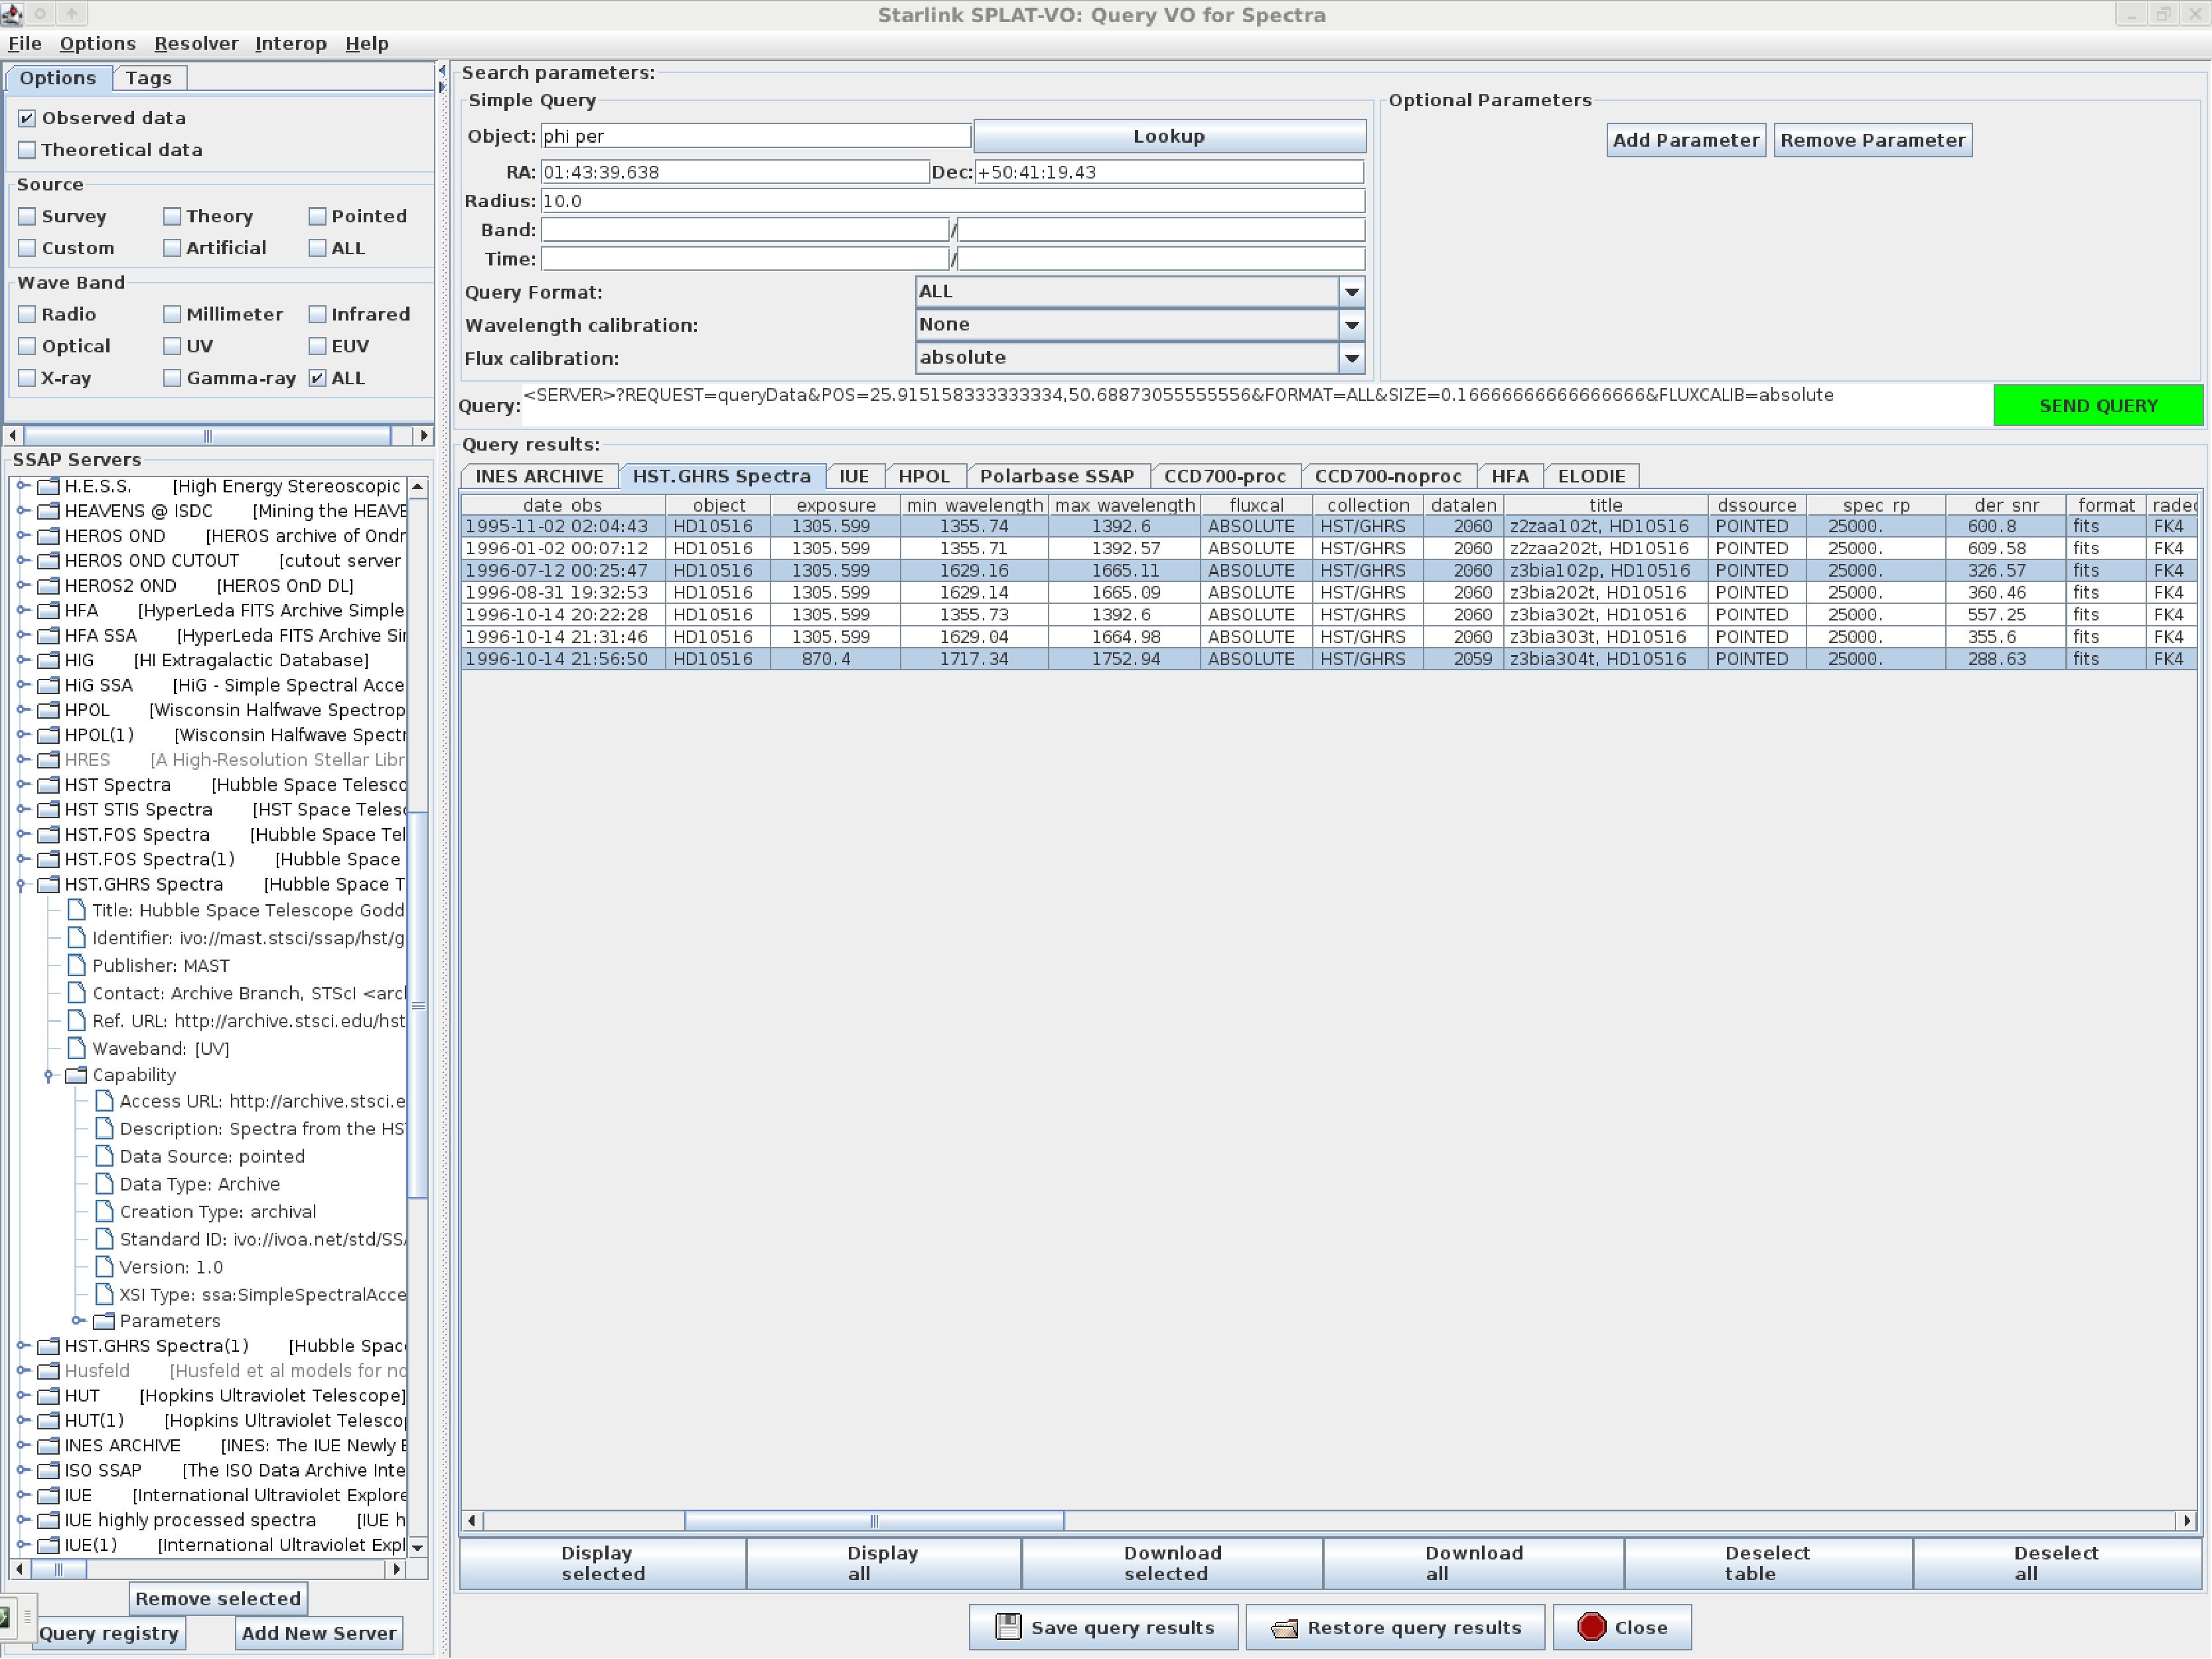
\includegraphics[width=0.8\textwidth]{hst_query.pdf}
\caption{The SSAP query for absolutely flux calibrated  spectra of $\Phi$~Per with results obtained from HST GHRS service}
\label{fig:hst_query}
\end{center}
\end{figure*}


\begin{figure*}[t]
\begin{center}
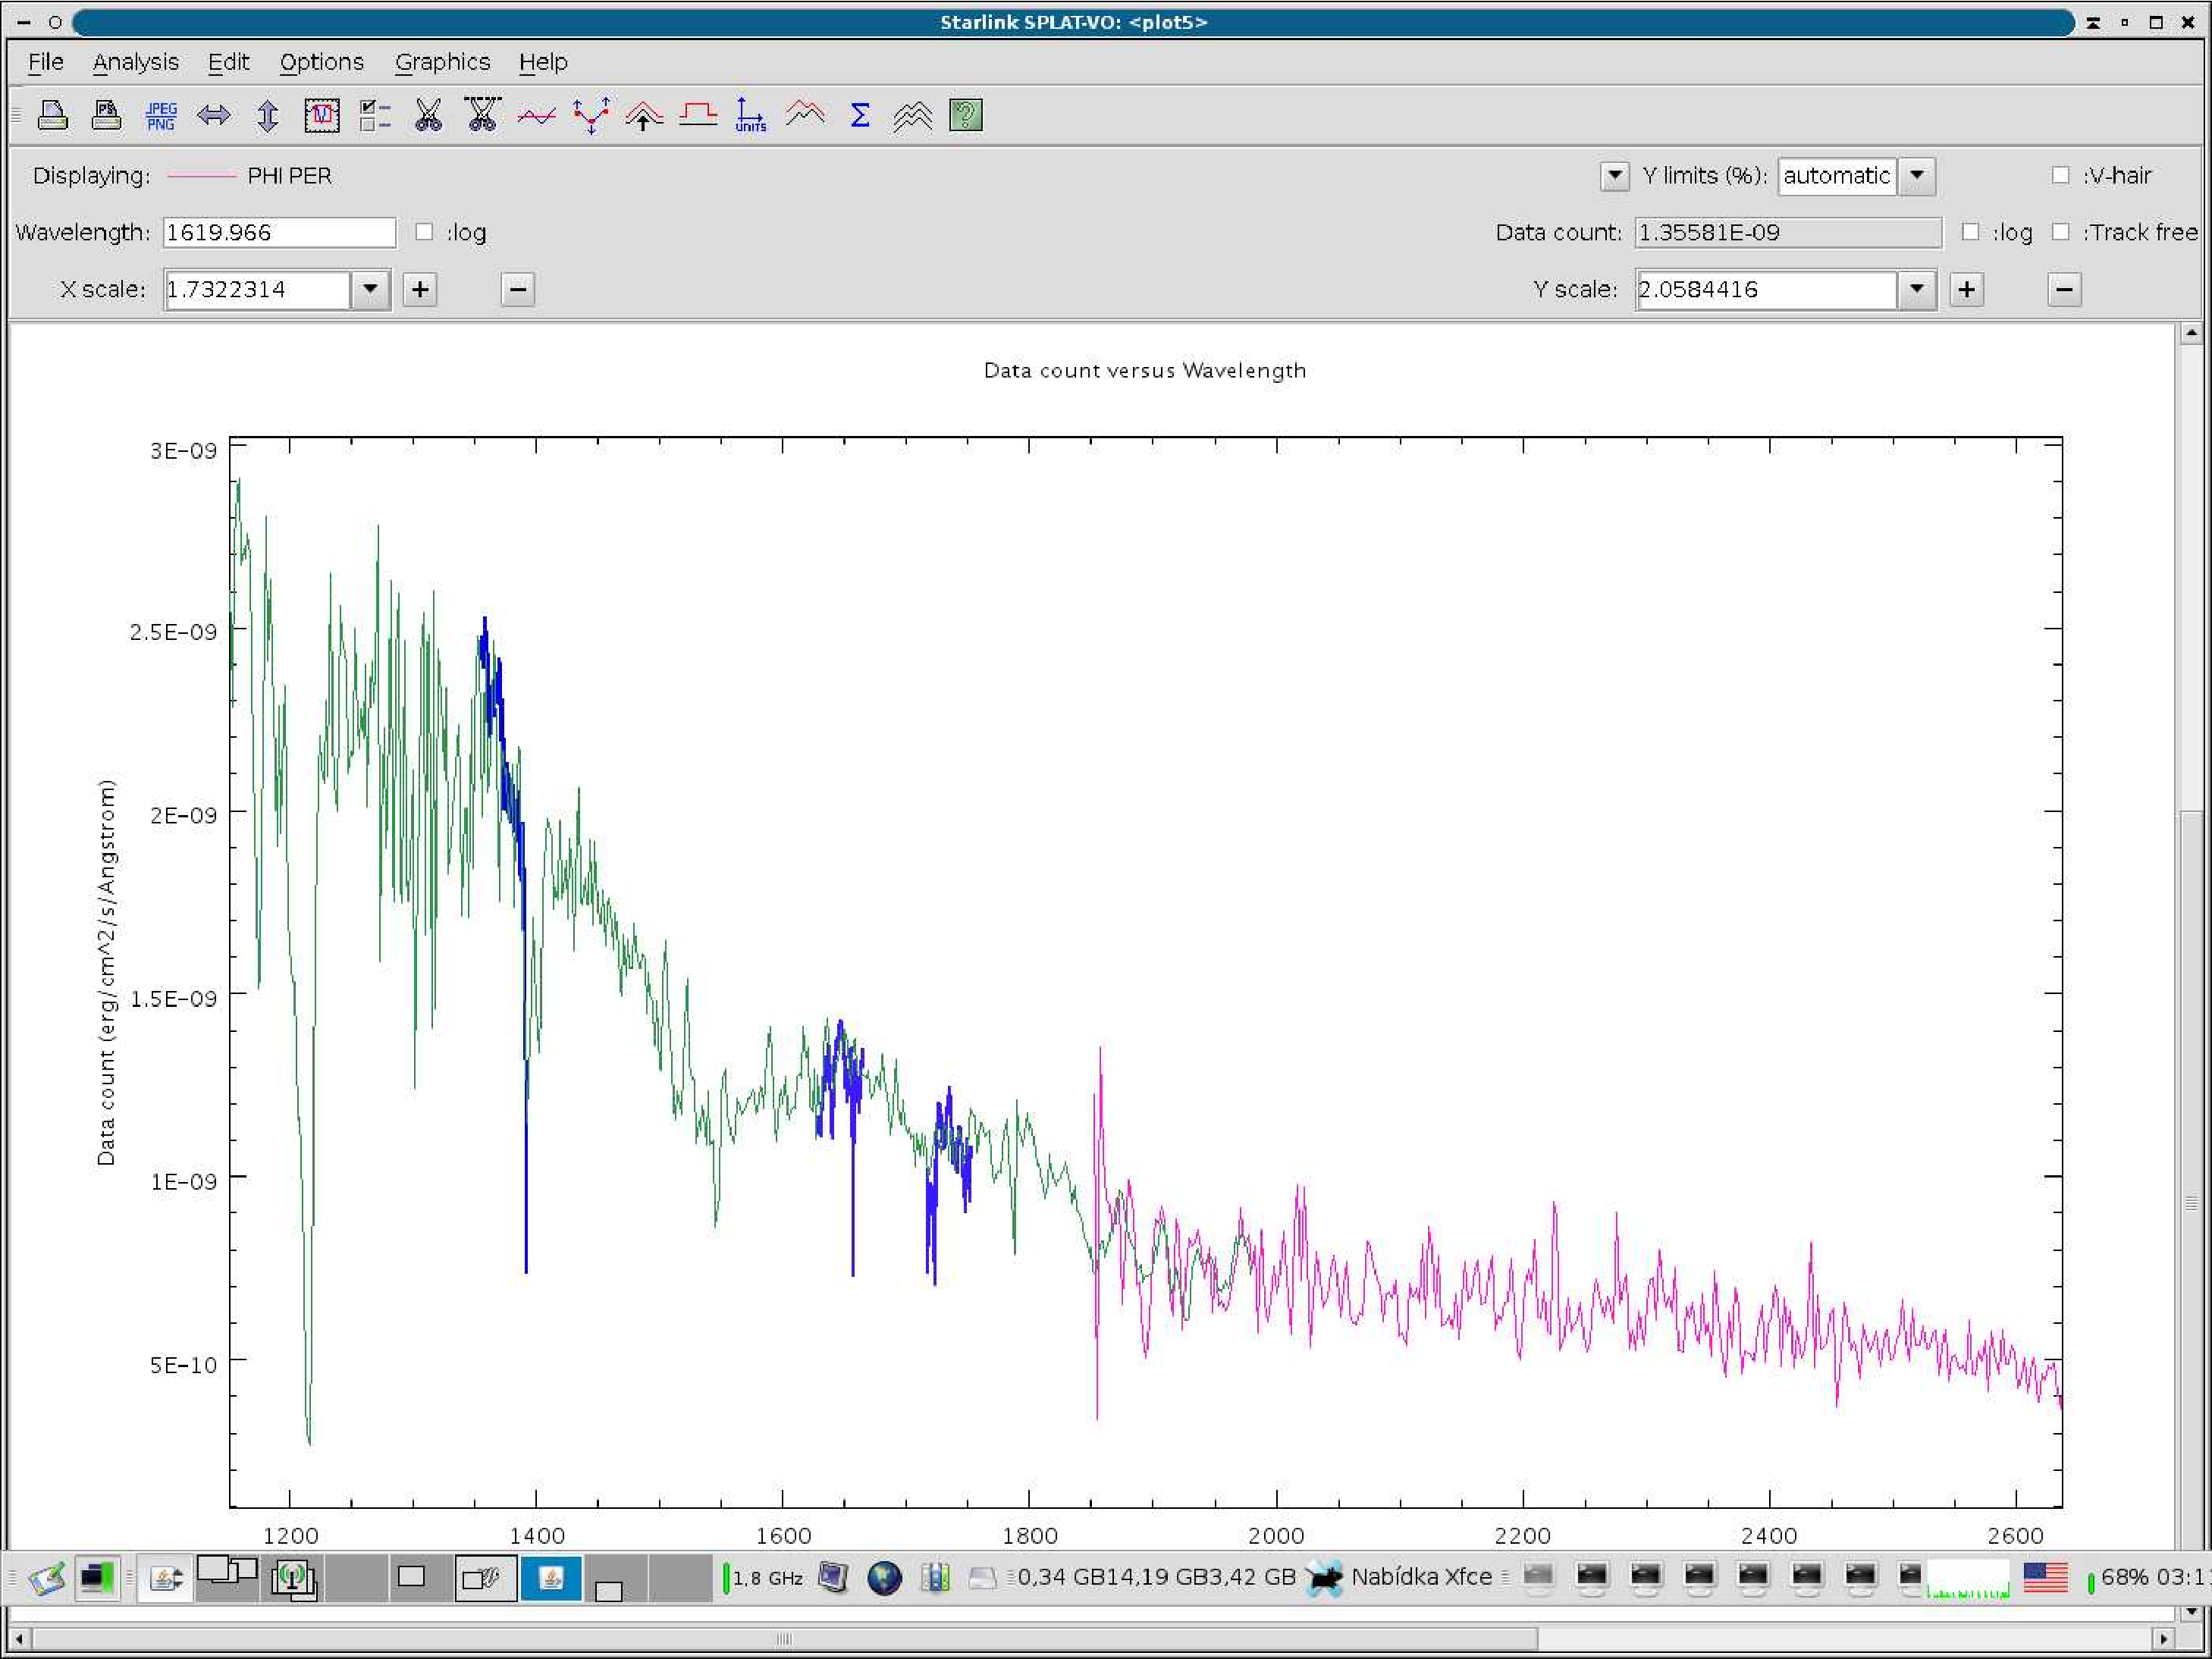
\includegraphics[width=0.8\textwidth]{iuehst2.pdf}
\caption{Composite plot of UV spectra of $\Phi$~Per from  HST GHRS spectrograph  selected in query on Fig.~\ref{fig:hst_query} and IUE low resolution spectra selected earlier}
\label{fig:iuehst2}
\end{center}
\end{figure*}



\subsection{ Theoretical Spectra Access}

In a similar way like observational spectra  are obtained synthetic spectra
from the libraries  available in VO (e.g., Kurucz models, Rauch's non-LTE model
spectra, TLUSTY hot stars, Salpeter, Dusty). They are selected by radio
button, which  changes the role of parameters used to query. The extended
protocol called Theory-SSAP \citep[hereafter TSAP;][]{ssap} uses  the various
physical parameters like $T_{\rm eff}$, $\log g$, metalicity etc. for query
instead of position, wavelength regions and time range. Unfortunately, there do
not exist obligatory metadata for all required physical parameters, so the user should try
himself what is available on given server.  The user than has to individually
select suitable spectra from multidimensional table combining all the
parameters ranges required.  The Fig.~\ref{fig:TSAP-query} and
Fig.~\ref{fig:TSAP-plot} shows the query and result of selection of several Kurucz models for
Vega.


\begin{figure*}[t]
\begin{center}
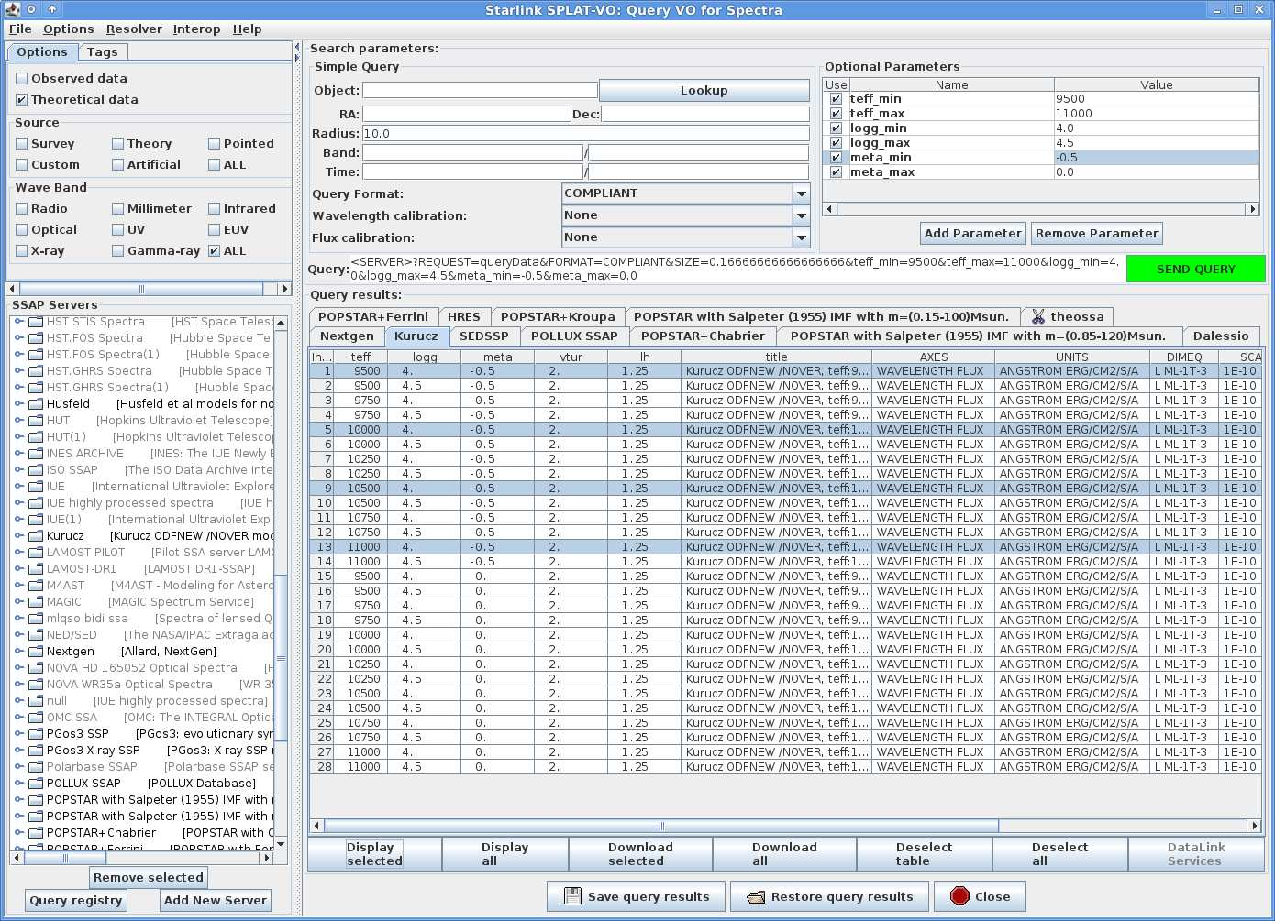
\includegraphics[width=0.8\textwidth]{TSSA-query.pdf}
\caption{TSAP Query for Vega-like Kurucz models. Note the additional parameters needed.}
\label{fig:TSAP-query}
\end{center}
\end{figure*}


\begin{figure*}[t]
\begin{center}
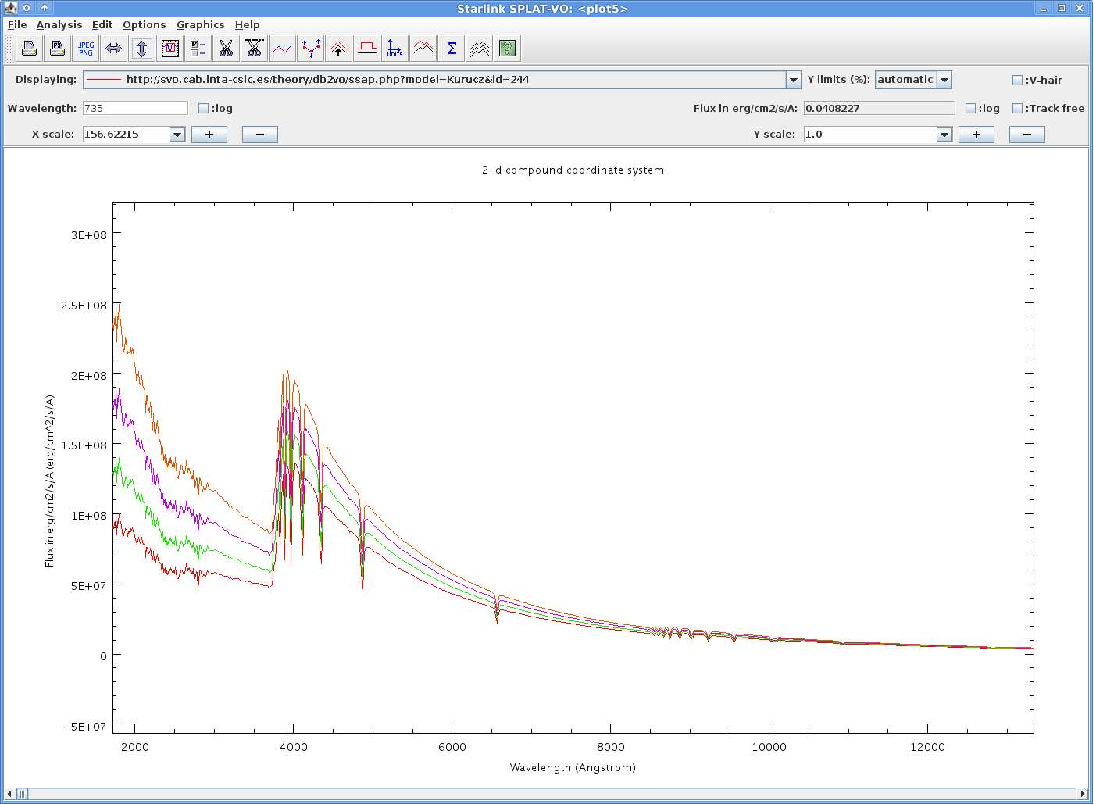
\includegraphics[width=0.8\textwidth]{TSSA-plot.pdf}
\caption{Zoomed plot of Vega-like Kuruz models manually selected in previous
TSAP Query window (see Fig.~\ref{fig:TSAP-query}). }
\label{fig:TSAP-plot}
\end{center}
\end{figure*}


%-------------------------------------------------------

\section{Recent Additions}


\subsection{Motivation}

As the VO evolves, adding new protocols and data models, SPLAT-VO
needs to evolve accordingly.  The further development of SPLAT-VO has
been continued by Margarida Castro Neves and Markus Demleitner at the
University of Heidelberg, and by and Petr \v{S}koda and David Andre\v{s}i\v{c} at
the Astronomical Institute of the Academy of Sciences of the Czech
Republic.

SSAP, as the name says, is a simple protocol, and has some limitations. Some
features like cut-outs or flux calibration, which are often needed, have to be
performed in a second work step after downloading the spectra. It is much more
efficient to have it done on-the-fly at the server and  to download the
spectra exactly as needed. To overcome the limitations of SSAP, the new
DataLink protocol \citep{datalink} was used. SPLAT-VO is one of the first
client implementations of DataLink, in this way also contributing to its
testing and development from a client point of view.

Besides SSAP, spectra can also be retrieved using the ObsCore data model
through Table Access Protocol(TAP)  \citep[known as ObsTap;][]{obstap}. Its implementation in
SPLAT-VO allows spectra to be retrieved also from ObsCore services, and
the ObsTAP ADQL \citep{adql} search offers a more powerful search
mechanism as well. The implementation of new VO protocols like ObsTAP
and DataLink have been done side-by-side with their server-side
implementation in DaCHS \citep[Data Center Helper Suite;][]{dachs},
developed by Markus Demleitner.

Also SPLAT-VO's user interface has been improved. An improved server
selection interface and SSAP search by metadata parameters are some of
the new features added, which are listed in the next subsections.

\subsection{New Features in VO Access}

\subsubsection{SSAP service selection}

In the earlier versions of SPLAT-VO a list of services was presented, and
the user could select the services to be queried, as well as remove
uninteresting services from the list. Information about the services
of interest had to be gotten from somewhere else, as the service
metadata was not used.  This simple server selection interface has
been exchanged by a more detailed selection, users can choose a set of
services that may contain data of interest, based on the services
metadata taken from the registry (data source, waveband).

There are two ways of selecting services. The first way is to choose
according to data source (survey, pointed observation, simulation...)
or waveband.  For example, the user wants to select services
containing pointed observation sources in optical wavelength, so this
can be selected in the interface and only the services which contain
this information in the metadata will be selected.  The other way is
useful in the case when users know exactly the services they want to
query, so they may create an own tag containing the chosen services,
and give it a name, such as ``My Favourite Services'', which will be saved
and loaded the next time SPLAT-VO starts.

This implementation relies on the metadata information from the
registry services, which should be correct and complete. Unfortunately
many services information from the registries are not complete, or not
correct, what we hope will be fixed in the future.



\subsubsection{Manual addition of SSAP services}

SPLAT-VO gets its list of SSAP services by querying a registry
service.  A new function has been added to allow inclusion of a new
service that is not (yet) registered. This is useful to access a
local, not public service, or to test a service before it's included
in the registry.

\subsubsection{Metadata parameters query}

In it's original version, SPLAT-VO contained just a simple cone search using
the SSAP obligatory parameters (RA, DEC, band, time, data format) and later
added wavelegth and flux calibration state, although many other metadata is
available on servers.  Now SPLAT-VO retrieves also the metadata parameters for
each server, and a new user interface allows users to chose metadata
parameters and their values to perform more detailed queries.  This is
especially interesting when querying theoretical spectra by TSAP, which contain many
additional query parameters. Figure~\ref{fig:TSAP-query} shows the
use of additional metadata parameters.

\subsubsection{Simple HTTP authentication}

It can be used when data is published to the VO before it should be
publicly available. So the owner and a limited group of users can
access it before disclosure. The authentication can be done on a
service basis, where the whole service needs authentication to be
queried, or on a spectrum basis, i.e. only some of the spectra from a
certain service require authentication to be downloaded. In any case,
an username/password window will appear when needed.

\subsubsection{GetData and DataLink}

To overcome SSAP limitations and allow server-side processing of
spectra like cut-outs, or format conversions, a protocol called
getData has been developed. After successful implementation and
testing on SPLAT-VO, the work on getData has been stopped. It has been
decided to go on implementing this features using the new Datalink
protocol, which will probably be implemented by several services in
the future, and can also be used in different cases.  Datalink
resources can provide links with several ways to access the data,
covering getData functionality and more. This feature is still in test
phase, as the DataLink protocol is still in development.

When parsing the service response from a SSAP query, which is in form
of a VOTable, SPLAT-VO looks for a \texttt{RESOURCE} element of type \texttt{service}.

An example is shown below:

{\tiny
\begin{minipage}{\textwidth}
\begin{verbatim}
<RESOURCE ID="aeoadowdpudn" type="service">
  <GROUP name="input">
    <PARAM arraysize="*" datatype="char" name="ID"
    ref="ssa_pubDID" ucd="meta.id;meta.main" value="">
      <DESCRIPTION> The pubisher DID of the dataset of interest
      </DESCRIPTION>
    </PARAM>
    <PARAM arraysize="*" datatype="char" name="FLUXCALIB"
    ucd="phot.calib" utype="ssa:Char.FluxAxis.Calibration" value="">
      <DESCRIPTION>Recalibrate the spectrum.  Right now, the only
      recalibration supported is max(flux)=1  ('RELATIVE').</DESCRIPTION>
      <VALUES>
        <OPTION name="RELATIVE" value="RELATIVE"/>
        <OPTION name="UNCALIBRATED" value="UNCALIBRATED"/>
      </VALUES>
    </PARAM>
    <PARAM ID="aemoogtm" datatype="float" name="LAMBDA_MIN"
    ucd="par.min;em.wl" unit="m" value="">
      <DESCRIPTION>Spectral cutout interval, lower limit</DESCRIPTION>
      <VALUES>
        <MIN value="3.3696e-07"></MIN>
        <MAX value="8.7665e-07"></MAX>
      </VALUES>
    </PARAM>
    <PARAM ID="appadowdpudn" datatype="float" name="LAMBDA_MAX"
    ucd="par.max;em.wl" unit="m" value="">
      <DESCRIPTION>Spectral cutout interval, upper limit</DESCRIPTION>
      <VALUES>
        <MIN value="3.3696e-07"></MIN>
        <MAX value="8.7665e-07"></MAX>
      </VALUES>
    </PARAM>
  </GROUP>
  <PARAM arraysize="*" datatype="char" name="accessURL" ucd="meta.ref.url"
  value="http://dc.zah.uni-heidelberg.de/flashheros/q/sdl/dlget"/>
</RESOURCE>
\end{verbatim}

\end{minipage}
}

The GROUP element with name \texttt{input} contains the input
parameters that will be returned to the server.  It must contain an ID
parameter, which refers to the metadata that identifying the required
spectra (normally the \texttt{pubDID} parameter).  The other parameters in
this group are the ones for which the users can set values that will
be sent to the service as a request. The \texttt{accessURL} parameter defines
the service URL to which this request has to be sent.

In the SSAP response to a query, the services supporting DataLink will
be marked with the  ``\ding{34}''  icon. When one of these services is
selected, the user can activate the DataLink feature by clicking on
the button with same name. When activated, a window with a form to
enter values to the DataLink parameters will appear. While this window
is activated, every spectrum selected and downloaded from this service
will be processed according to the chosen parameters. When
de-selected, the spectra will be downloaded as they are in the SSAP
service, without processing.

In the case described above, the DataLink resource is in the query
response from the SSAP service. In another case, after a query, some
services return a list of spectra pointing not to the spectral data to
be retrieved, but to a VOTable containing only DataLink information
with the links to the URLs of the data. This DataLink resource has
then to be parsed by SPLAT-VO in order to retrieve the selected spectrum.

\subsubsection{ObsTAP}

Besides SSAP, spectra can be retrieved using ObsTAP. This service uses
the Table Access Protocol (TAP) to query metadata from the Observation
Data Model Core Components (ObsCore). Currently there are few services
implementing it, and SPLAT-VO implementation is ongoing.  ObsCore
provide standard metadata attributes that can be used, through the
ADQL query language, to perform more extensive and detailed queries
than in the case of SSAP data discovery.

In the current SPLAT-VO implementation, users can select ObsCore in the
main SPLAT-VO window. The ObsCore browser window will appear, which is in
part similar to the SSAP browser window. The user can chose either a
similar cone search interface like the one in SSAP, or a (still)
rudimentary ADQL interface where some parameters can be set. For more
advanced queries, the user can directly edit the ADQL
expression. After sending the query the results tables will be
displayed, which are in functionality similar to the SSAP browser
window. For the TAP query SPLAT-VO uses STARJAVA's TAP functions written
by Mark Taylor.


\subsubsection{Visualizing Light Curves using  SSAP}

As the proper standard for displaying photometric light curves or time series
of other variables is not so far established by IVOA, there were several
attempts to exploit the visual similarity of spectra and light curves
pretending the spectral axis is the temporal one.  So the SSAP was
successfully used as a transport protocol for delivering light curves in
binary table format. In principle the table may contain many columns displayed
as dependent variable against the various time axes with interactive menu.
The current limitation only requires the time axis expressed as floating point
variables, which limits the possibility of using strings (e.g., dates, time
stamps or even the names of CCD images used to extract given photometric point
on light curve.  An example in Fig~\ref{fig:OGLE-SC7-127550_query} shows the
query and corresponding light curves obtained  (Fig.~\ref{fig:OGLE-SC7-127550_plot})  from
Ond\v{r}ejov Southern Photometry Survey \citep{skoda_adassxxiii} ongoing on
at Danish 1.5m telescope DK154.



\begin{figure*}[t]
\begin{center}
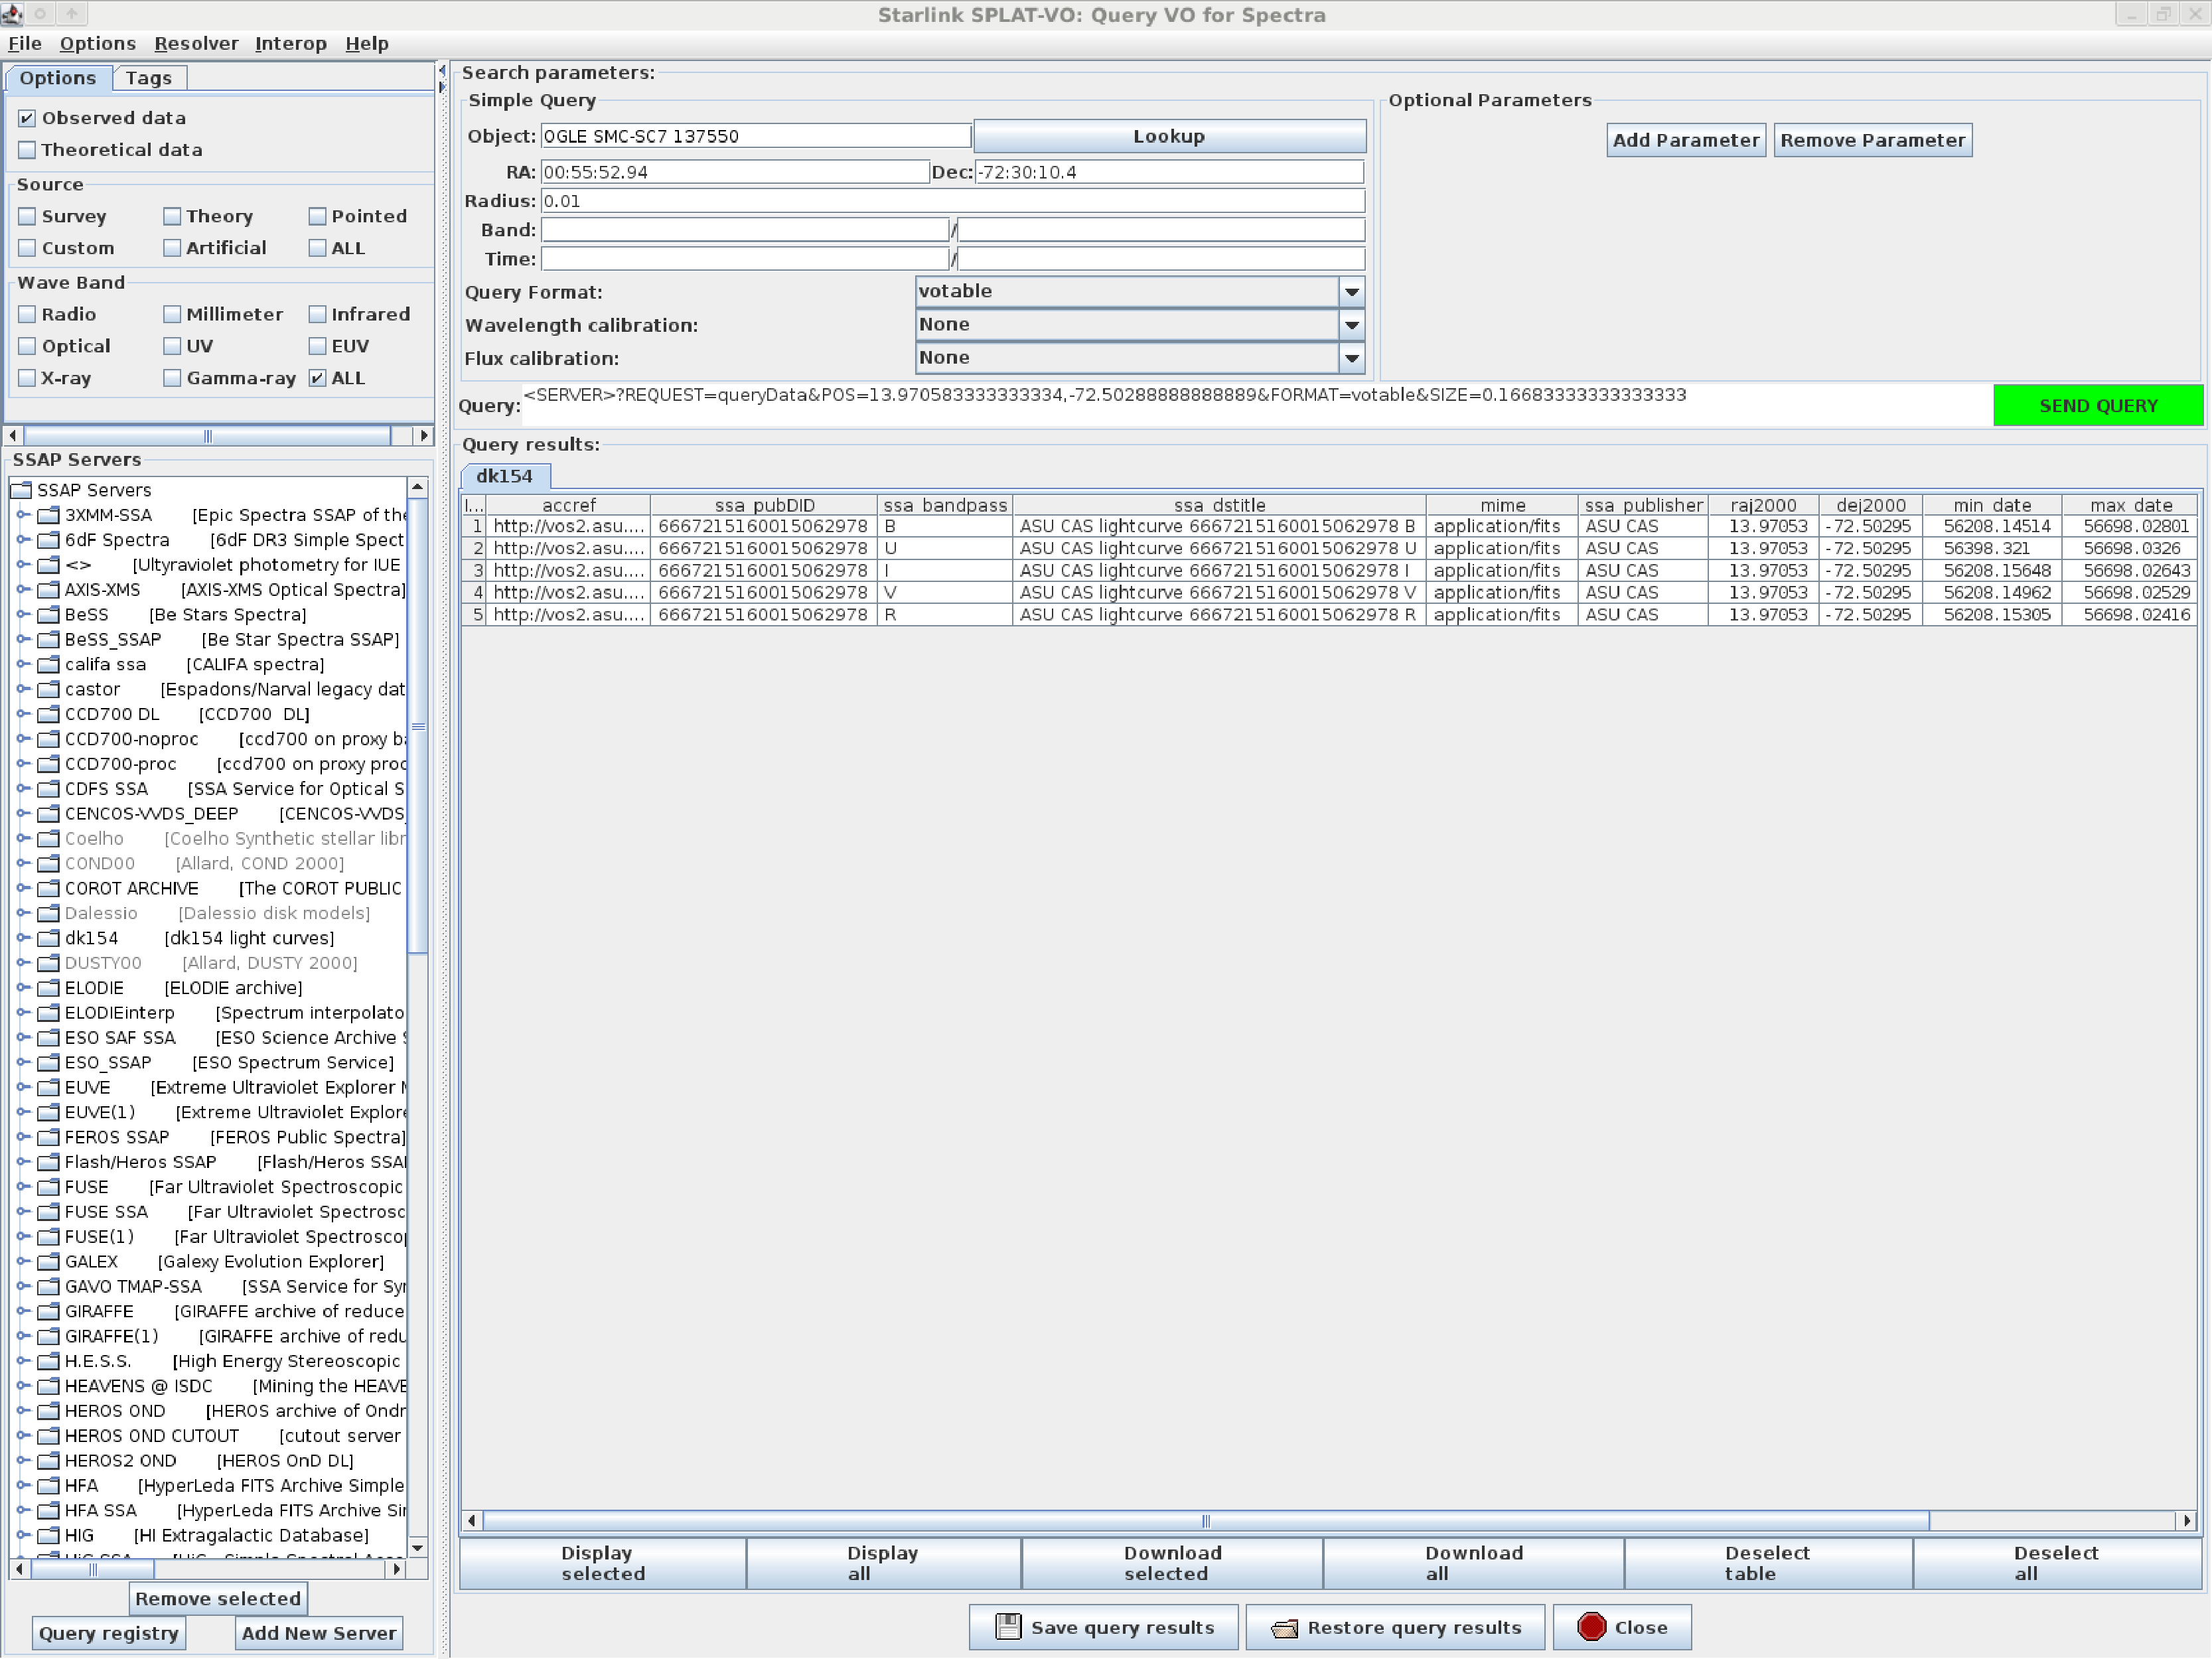
\includegraphics[width=0.8\textwidth]{OGLE-SC7-127550_query.pdf}
\caption{Example of using SSAP for obtaining multicolour light curves from OSPS}
\label{fig:OGLE-SC7-127550_query}
\end{center}
\end{figure*}

\begin{figure*}[t]
\begin{center}
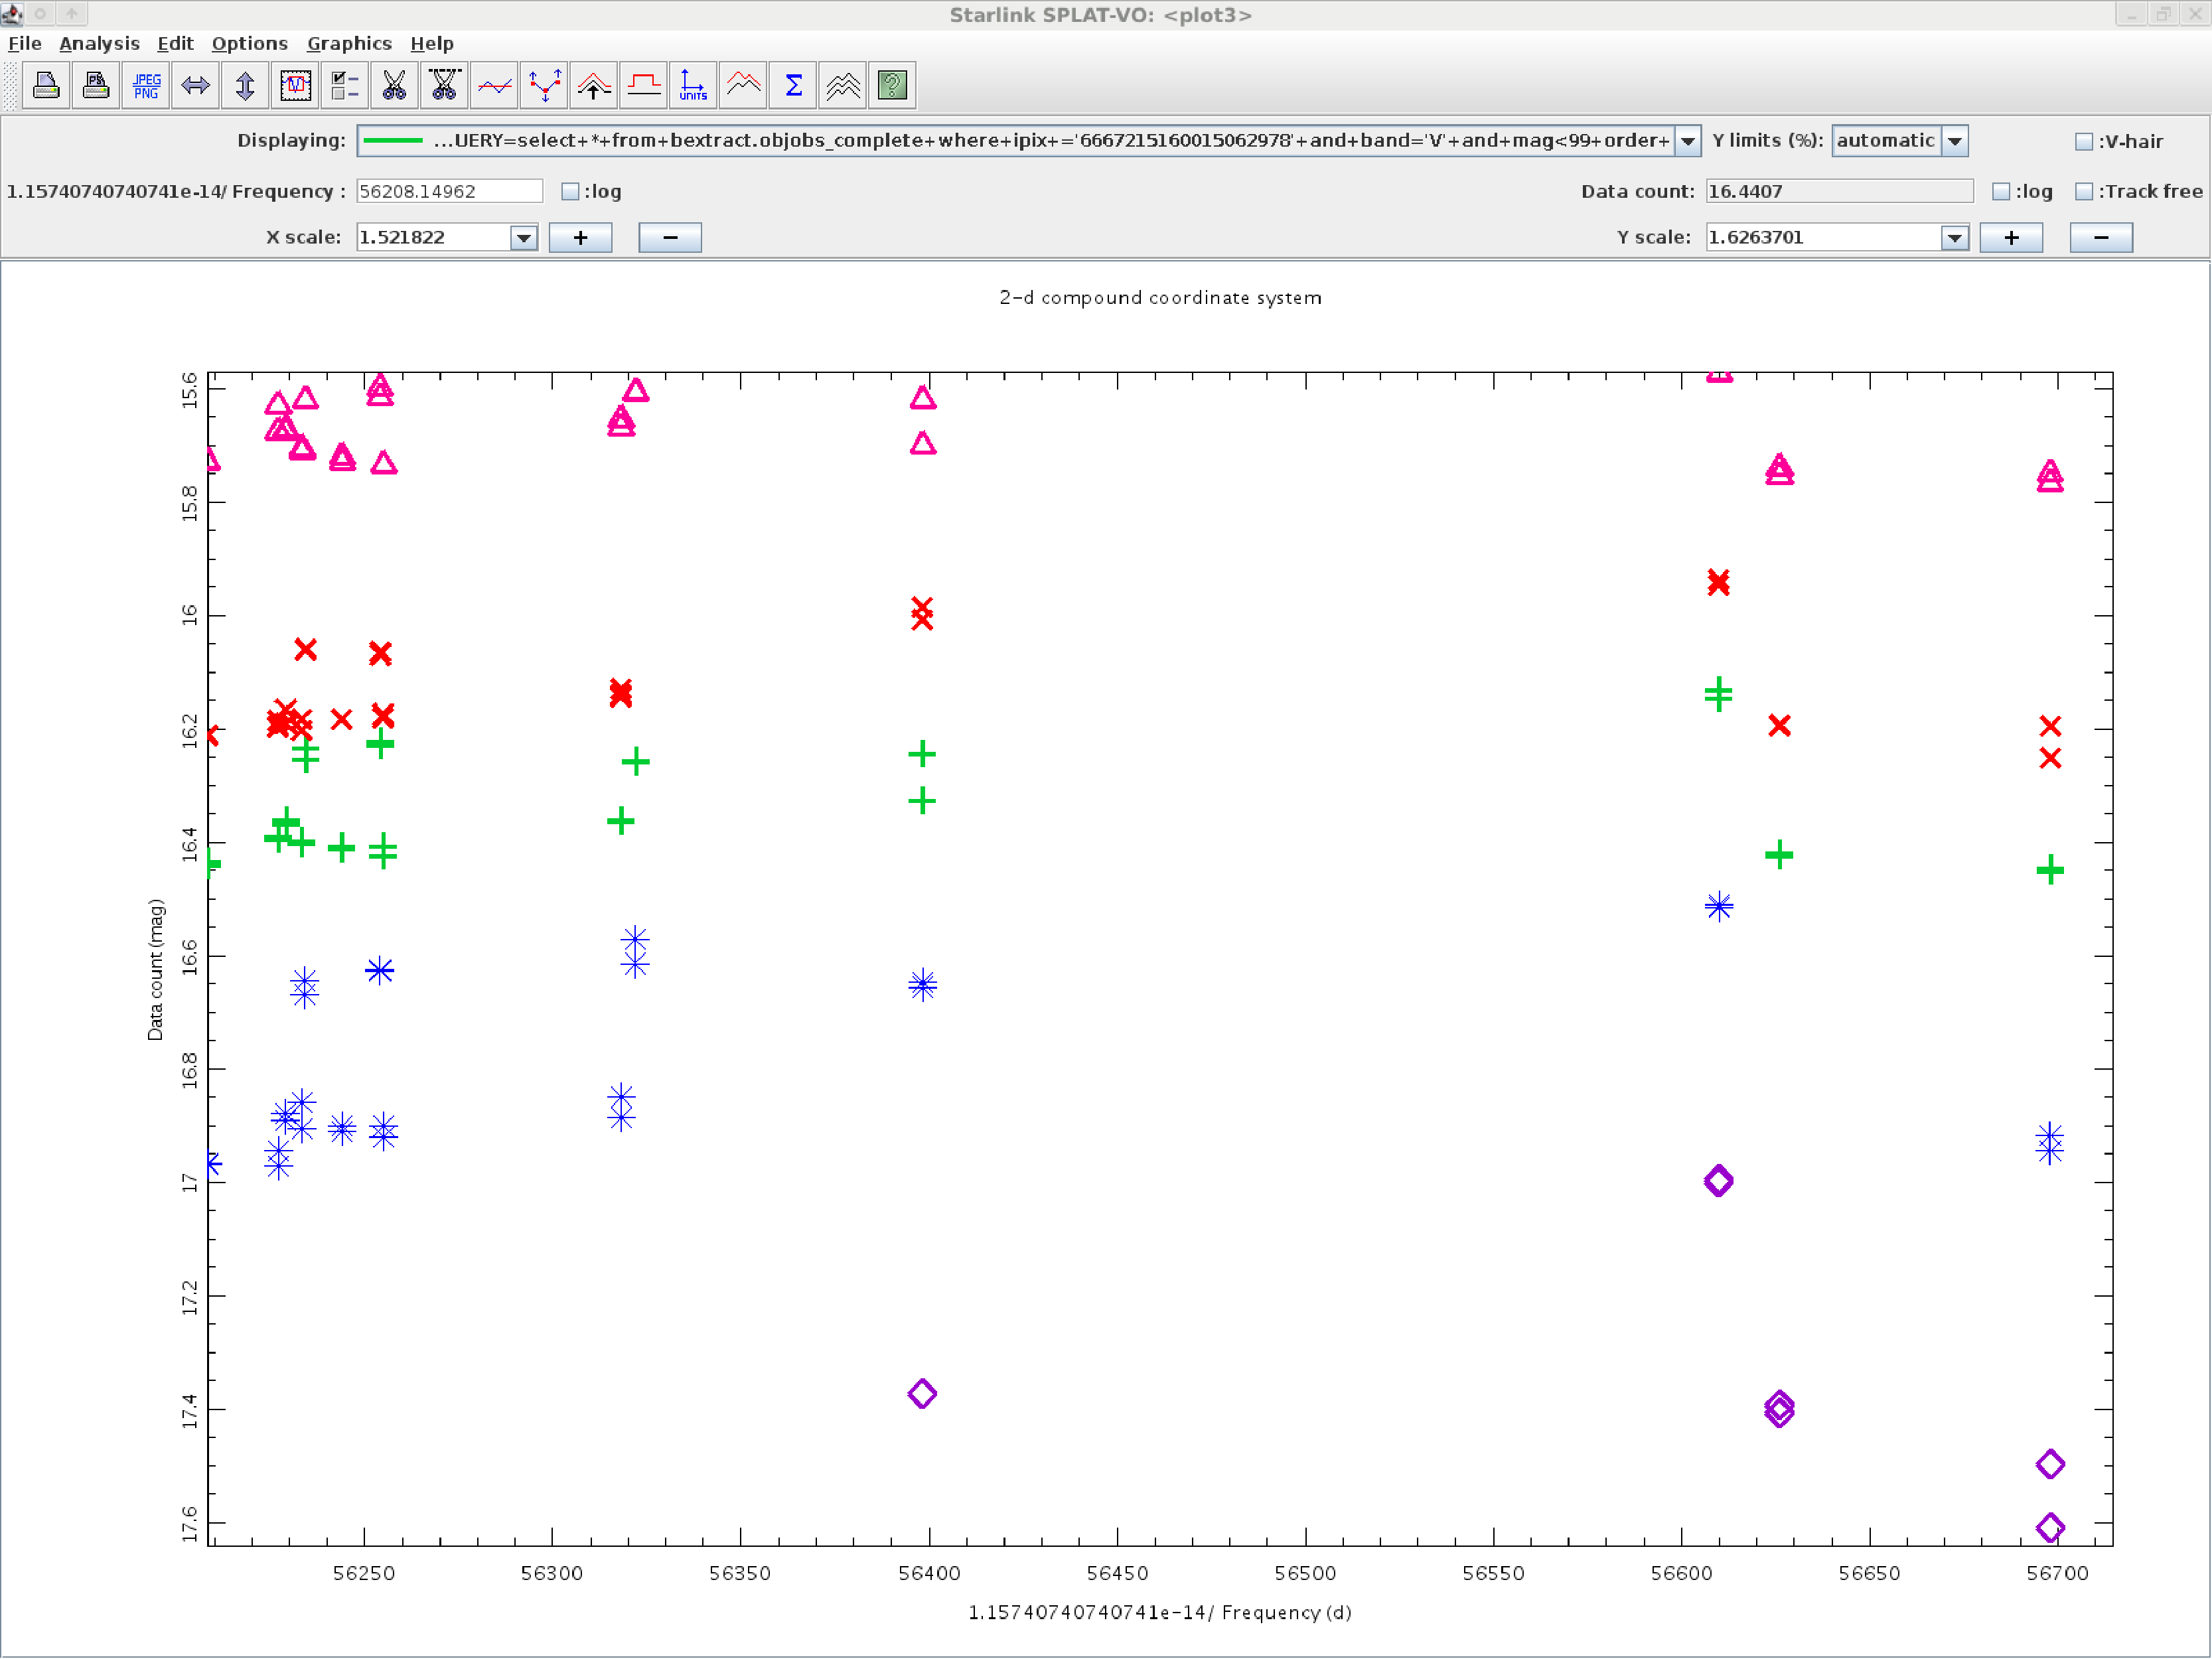
\includegraphics[width=0.8\textwidth]{OGLE-SC7-127550_plot.pdf}
\caption{Multicolour light curves of Cepheid OGLE-SC7-127550 from
  OSPS. The manual modification of default line type into various
  markers and flip of vertical axis was applied on data obtained by
  experimental SSAP light curve protocol using query from
  Fig.~\ref{fig:OGLE-SC7-127550_query}. The measurements in
  Johnoson-Cousins filters correspond to U (diamonds), B (asterisks),
  V (pluses) R (crosses) and I (triangles).  }
\label{fig:OGLE-SC7-127550_plot}
\end{center}
\end{figure*}

\subsection{New Features in Spectral Analysis}

\label{davids_functions}
For better analytic capabilities and user comfort in
general, were added \citep{and146bcthesis} to SPLAT-VO following features:

\subsubsection{Saving Spectra Stack in Multi-extension FITS format}

Previous versions of SPLAT-VO were able to save its global list of spectra only to
their native binary format, which was in fact the memory dump of spectra
objects. But sometimes, there may be a need to save that list to a more
universal, standardized format. For example, SPLAT-VO allows to perform many
operations on spectra, which results in a new spectrum object that is added to
a global list of spectra (e.g., cutting a part of spectrum). Saving the list of
such spectra to a standardized format would then allow its opening in another
tool and continuing to work with it in a way the SPLAT-VO wasn't designed to.
This may be helpful for preparation of large list of normalized line profiles
for Fourier disentangling or asteroismology studies.

Therefore, SPLAT-VO now allows the user to save the global list of spectra to a
much more universal FITS format, where every spectrum  is represented by its
own (IMAGE) extension.  The only disadvantage compared to the proprietary
format is that it won't keep the settings like colour or strength of the lines
or type of symbols used for points etc., since these information  are not
standardized for FITS.


\subsubsection{Visual Spectrum Selection and Highlighting}

In the earlier versions of SPLAT-VO, when the user worked with multiple
spectra in one common plot window, he  had a limited possibility of
selection just one of them for further actions. Selection of, for example, noisy
spectrum and its deletion from plot window could be done only by
trial-and-error procedure and therefore quite problematic and time-wasting.

We improved this and now when the user clicks on a spectrum in global spectra
list, SPLAT-VO will automatically select the closest spectrum to the cursor
position and  the spectrum gets immediately highlighted in all plot windows
that it is opened in. The highlighting has a form of a few-seconds blinking in
an inverted colour and is performed sequentially (highlighting in one plot
window comes after the previous one is finished), which gives to the user a
perfect sequential overview of the spectrum's plots.

\subsubsection{Cut window: saving the ranges}

In the 'Cut regions from spectrum' window, user could simply read
ranges of regions from a local file (feature available under 'File'
menu). But what if he made a visual selection of ranges from a
currently plotted spectrum and wanted to save it to a local file?

Since now, SPLAT-VO can save the currently defined
ranges to a local file (feature is available under 'File' menu) in the
same format as the reading feature expects, that is one range (with a
white space between its beginning and ending value) per line:

\begin{quote}
\small
\begin{verbatim}
# Generated by SPLAT-VO

# Range 1
8601.177 8621.531

# Range 2
8729.026 8748.744
\end{verbatim}
\end{quote}

\subsubsection{Cut window: performing on multiple spectra}

And cutting regions from spectrum again: until now, when user defined
all the wanted regions and performed the cut action, SPLAT-VO cut the
regions only from the currently active spectrum.

This window newly possess a table of all
currently plotted spectra in the corresponding plot window. User then
can select multiple of it (buttons for selecting and deselecting all
the spectra are of course there as well) and perform a cut (or any
other action in this window) on all the selected spectra.

\subsubsection{Display of All  spectra received by SAMP to the same  window}

In the previous versions of SPLAT-VO, all spectra received via the SAMP
protocol got opened in their own plot windows. Very often, it would be
necessary for comparative analysis to have them plotted in the same
window, but for this, the user had to do it manually.

SPLAT-VO is now able to do this
for the user automatically. We added new checkbox under the
'Interoperability' menu that can be used to switch between the previous
state (each spectrum to its own plot window) and plotting all the
spectra received by SAMP to their common plot window. This feature
can be of course turned on and off several times during the runtime,
so it allows to plot one bulk of spectra received by SAMP to one
window and another bulk to another window.

\section{Future plans for SPLAT-VO}

The goal of the developers is to keep SPLAT-VO up-to-date with the
newest IVOA Standards, many times testing and contributing to the
development of standards. Besides that, to keep improving the
visualization and scientific data analysis part to meet scientists
needs.  Some of the items listed below are already being worked on,
some others are being planned. It's also important for the developers
to get feedback from the users community on which additions could be
useful.

\subsection{New science and data functions}
\begin{itemize}
\item Automatic matching of line identifiers to spectrum;
\item Selection of spectra from data cubes,
\item Complex graphics attributes bound to individual spectral collections, Changes on kernel - work with stack of spectra together (e.g., cutouts, fitting )
\item Dynamic spectra - evolution of spectra profiles in time (gray scale representation)
\item Automatic continuum normalization algorithm to apply on all spectra received from servers not supporting it
\
(In principle folding with phase given period.)
\item Support for exporting the global list of spectra to another types of FITS extensions and other formats, like VO-Table.
\item Access to all extensions and its metadata in FITS received via SSAP protocol.

\end{itemize}

\section{Lessons learned}

During the development of SPLAT-VO a number of lessons have been
learned that may affect future developments of similar tools. In this
section we summarize these issues.

\subsection{Using JNI versus ``pure'' Java}
\label{sec:jniast-lesson}

The question should probably be asked if using a JNI wrapper to the
AST library was a good choice or not. As with most things, we believe
this was a good idea and also bad. The judgement of how bad depends on
how the ultimate cost benefit analysis works in the longer term, but
either way it is difficult to deny that a pure Java solution would
have been preferable.

The positives of this choice are that it made the development of
SPLAT-VO possible on useful timescales as we were able to immediately
benefit from all the work that had gone into the AST library, as AST
is very much more than just a system for handling coordinates and
units. It also insulates against the often messy need to parse FITS
headers and offers the ability to transform easily between all
compatible coordinates and units. Even today some 15 years later, AST
is still believed to be a class leader in these areas.

Avoiding this work was also pragmatic as a re-write into Java would
have been a lot of work that the effort just wasn't available for and
still isn't. In the intervening years there have also been new
features added to AST, such as the dual-sideband support, which was
vital for submillimeter work, and the adoption of SPLAT by the
JAC. The development of SPLAT has also been a useful testing ground
for the development of AST itself (like the introduction of thread
safety, so not just the handling of spectral coordinates), closing a
virtuous circle.

The downsides are only the obvious ones, not having a pure Java
solution compromises the portability, so we need to make an additional
effort for all the supported platforms. There is also the non-trivial
time writing the JNI layer itself takes. Writing JNI interface code is
more challenging than those more commonly found for scripting
languages.

\subsection{Open sourcing from the beginning}

The decision was made very early on for the SPLAT source code to be
made publicly available, first via CVS on a Starlink server, then via
Subversion on a Joint Astronomy Centre server and finally using \texttt{git}
on Github. We feel that this openness contributed directly to the
software being picked up by the GAVO project, saving the application
from stagnation once the direct funding for it was dropped.

\subsection{Local spectral line catalogues are not sufficient}

Currently SPLAT-VO uses a local text file containing molecular
transitions that are thought to be of interest and allows the user to
provide external lines via a text file of a similar format. The
internal list is dominated by sub-millimetre lines required by the
JCMT. Even so, the list of lines was never sufficient and astronomers
continue to ask for more obscure transitions to be included. A local
line catalogue is an excellent back up but it is also necessary to
look up catalogues from remote services. The ALMA-OT
\citep{2013ASPC..475..373W} works in exactly this way with much
success. This feature will be added in the future using the Simple
Line Access Protocol (SLAP) that will allow for retrieval of line
lists from big world-wide atomic and molecular database such as NIST
\citep{NIST_ASD,2012APS..DMP.D1004K,2004JPCRD..33..177L} and all the
databases from the VAMDC consortium \citep{2011BaltA..20..503K}.


\subsection{SPLAT-VO in data reduction pipelines}

Interactive user interfaces are very powerful but a number of issues
become apparent when reduction and analysis facilities are directly
integrated into an application where automation is a secondary
concern.  At the James Clerk Maxwell Telescope SPLAT replaced the
SPECX package \citep[][\ascl{1310.008}]{specx} which had been
developed for interactive command-line use whilst supporting a
scripting language to allow for bulk processing of spectra. With SPLAT
the promise of beanshell support was never able to overcome some key
difficulties associated with automation. There are two scenarios for
automation. The first is for an astronomer to record the steps taken
manually in reducing or analysing a spectrum and then replay that
analysis on many other spectrum. The second scenario is to allow key
algorithms to be made usable in a pipeline environment with the GUI
disabled. For the JCMT heterodyne pipeline
\citep{2008ASPC..394..565J,JennessACSISDR} all efforts at algorithmic
enhancement were focused on individual Starlink applications such as
KAPPA \citep[][\ascl{1403.022}]{sun95}, because it was unclear how
feasible it would be to add complex algorithms to SPLAT and make them
available through the pipeline. One of the interesting approaches
taken by GAIA \citep{2009ASPC..411..575D} was that all analysis
algorithms were called through a messaging interface such that they
could be used by the interactive GUI, from the command-line or from
the pipeline. This proved to be a very powerful approach but was not
available in the SPLAT design. Taking care to separate core algorithms
from interactive interfaces is an important design decision that has
long term ramifications for an application.

\subsection{Sub-millimeter units are complicated}

VOUnits \citep{vounits} standardisation is very useful but is not
sufficient for the majority of spectral line data that is encountered
by sub-millimeter astronomers. Sub-millimeter spectra are generally
calibrated in temperature rather than janskys and there are two
competing standards for handling the different calibration factors
that are involved in converting from such definitions as corrected
antenna temperature, main-beam temperature and antenna temperature
\citep{1981ApJ...250..341K,1989LNP...333..351D,2009tra..book.....W}. The
units alone do not tell you which temperature scale is in use and many
efficiency values are required when comparing spectra from different
telescopes. The situation is in dire need of standardisation efforts
and we simply had to ignore the issue in SPLAT.

\subsection{Service selection interface}

The new SSAP service selection interface, using more metadata
information from the services, is meant to help the user to choose the
specific services needed and to avoid making unnecessary queries and
downloading data which is not needed. Sometimes too much detail may
lead to confusion, especially if the service information from the
registries is often incomplete. If the data is not there as it should
be a detailed interface won't do much. The current interface will be
redesigned in the future, probably simpler but more accurate. It has
been planned also to use RegTaP \citep{regtap} to look for spectral services, which
may provide easier handling.

\subsection{Tracking VO standards is hard}

SPLAT transitioned from a local analysis tool to a VO client during
the birth of the VO and witnessed an explosive growth of standards
during that time. One interesting outcome of this was that funding for
SPLAT became scarce as the VO grew and funds were diverted from
classical astronomy software development efforts. VO standards became
increasingly important and it was clear that support should be added
for SSAP and related standards although it was a struggle to
prioritise this effort as VO adoption was initially slow and
astronomers were not driving the initial support for these
facilities. SPLAT-VO is being updated to add support for standards
such as DataLink \citep{datalink}, ObsCore \citep{obstap} and RegTap \citep{regtap} as well as expanded units support with
VOUnits \citep{vounits} required to understand the metadata from these
services, but the VO standards will continue to evolve
as new versions are announced and new standards developed and it will
be a continuing struggle to remain compliant. There is a worry that
all of the development effort available to SPLAT-VO will be spent
simply on maintaining standards support and this will be at the
expense of supporting new analysis algorithms. This is a very
difficult balancing act and we can not expect the IVOA standards
process to stagnate purely to make life easier for applications
developers.


\section{Obtaining SPLAT-VO}

SPLAT-VO is released in a variety of ways, you can build it using the source
code, obtain it as part of a Starlink JAC release. Alternatively you can
install into your desktop using a standalone IzPack bundled version or run it
up using Java webstart.

The bundled standalone and webstart releases of SPLAT-VO are currently
available for the following desktops, Linux (32 and 64 bit), Mac OS X (32 and
64 bit Lion) and Windows XP and later (32 bit Java only). Previous versions
also worked on Solaris, Sparc and Intel, and OS X PPC.

The Starlink releases
\citep[e.g.,][]{currie_adassxxiii,2013ASPC..475..247B} are available
for Linux (32 and 64 bit) and OS X (Lion and Snow Leopard).

See \ascl{1402.007}\footnote{or \url{http://astro.dur.ac.uk/~pdraper/splat}}
for the main support site where links to these releases can be found.
Releases of recent GAVO developments are also available and these
developments will be merged into the main SPLAT-VO releases.

The source code for SPLAT-VO and its associated libraries is
open-source and available on Github at
\url{https://github.com/Starlink/starjava}


\section{Conclusions}

The SPLAT-VO is the very powerful tools for analysis of spectra
allowing immediate browsing of world-wide distributed archives as well
as detailed study of individual objects in whole electromagnetic
spectrum including building of SEDs. Its capabilities makes it an
ideal tools for analysis of astronomical spectra even in local mode
for the non-VO-aware astronomers, although the full productivity is
reached in the VO environment.  It has been under active development
promising soon the handling of light curves and data cubes Thanks to
joining the effort of developer of GAVO DaCHS server suite and
SPLAT-VO developers the SPLAT-VO is an ideal reference implementation
for testing new IVOA proposed standards, as required by IVOA rules for
pushing standards in the Recommendation phase.

\section*{Acknowledgements}

The initial work on SPLAT-VO was supported
by the now closed Starlink Project funded by the Particle Physics and
Astronomy Research Council and more recently by the Joint Astronomy
Centre, Hawaii, also funded by the Particle Physics and Astronomy
Research Council and more recently by its successor organisation the
Science and Technology Facilities Council.

The current work on SPLAT-VO by GAVO is supported by German Federal
Ministry of Education and Research, BMBF grant 05A11VH3 and the Czech
development is supported by grant 13-08195S of Granting Agency of the
Czech Republic and by the Czech project RVO:67985815.

We thank Mark Taylor, who added to
SPLAT-VO his SAMP library and created the VO Registry interface, and
Markus Demleitner who actively supports the new features in SPLAT-VO SSAP
and DataLink handling by the development of GAVO DaCHS server publishing suite.
We also thank Jan Wouterloot for his work testing the sub-millimetre
features of SPLAT.

\bibliographystyle{model2-names-astronomy}
\bibliography{acsplat}


%!!! explain what is OSPS and cite ADASS article !!!
%bc thesis of Andresic




%\begin{figure*}
%\begin{center}
%\includegraphics[width=0.8\textwidth]{}
%\caption{}
%\label{fig:}
%\end{center}
%\end{figure*}



\end{document}
